\documentclass[fancy,11pt,titlestyle=display]{style/elegantbook}

\usepackage[underline=true]{pgf-umlsd}

\usepackage{hyperref}
\hypersetup{
    colorlinks=true,
    linkcolor=blue,
    filecolor=magenta,      
    urlcolor=blue,
}

\title{Cloud Computing}
\subtitle{Stony Brook CSE 356}
\author{Michael Ferdman and co.}
\institute{Stony Brook University}
\date{\today}
\version{0.2a}

\extrainfo{Go Seawolves!}

\logo{logo.png}
\cover{cover.jpg}

\begin{document}

\maketitle
\tableofcontents
\clearpage
\thispagestyle{empty}
\mainmatter
\hypersetup{pageanchor=true}

\chapter*{Preface}
\addcontentsline{toc}{chapter}{Preface} 
\markboth{Preface}{} 

This is a collaboratively edited collection of notes from the CSE356: Cloud Computing course from the Department of Computer Science at Stony Brook University.

\chapter{Cloud Computing Basics}

\begin{introduction}[Topics]
\item Clients and Servers
\item Server Hardware
\item IP and NAT
\item IaaS
\item Security Groups
\end{introduction}

\section{Servers and Clients}

\begin{definition}{Server}{}
A server is a computer/software that processes requests (i.e., receives data from a client or another server) and delivers data based on those requests.
\end{definition}

\begin{definition}{Client}{}
A Client is a piece of computer hardware or software that accesses a service made available by a server.
\end{definition}

\section{Server Hardware}

Server hardware runs a piece of software called a 'server'.
Usually dedicated machines designed to run 24/7, because if it's powered down then access is gone. Nowadays, bigger companies are able to host backups in various data centers to provide for all possible contingencies.

It used to work as follows:
designate space in a closet
put a machine in
plug in a network cable
Nowadays, we have more secure and reliable rooms called datacenters
but they are prohibitively expensive for individuals.

To overcome this, we have the ``cloud'' computing model, where a large service provider builds and maintains the datacenter, including purchasing the server hardware, and handles the networking.  then the service provider rents out server hardware to organizations that want to host online services, deciding pricing on the amount of resources used (and for how much time they are used).

economical model for small organizations, because to start out they get ``limitless'' cloud infrastructure without CapEx.  maybe good for large organizations too because OpEx of datacenter is high and requires expertise (that organizations may just be willing to pay for/rent instead of running themselves).

The way servers are stored in datacenters is by providing server racks (which originated from amplifier racks) to hold the servers in a compact space. The height of these servers would typically be described in U units in order to help with determining how many servers could fit in specified server racks.

\section{IP and Network Address Translation}

IPv4 is the old protocol (used to identify devices on a network), which is comprised of 32-bits. It is currently full, so there are two current alternatives:

\begin{definition}{IPv6}{}
The newest protocol, IPv6 is made up of 128-bits.
\end{definition}

\begin{definition}{NAT}{}
NAT maps a single IP address to a local network. This allow a single IP address to represent a whole entire network from outsiders and aid in security
\end{definition}

Public IPv4 address are separated into several different classes:
\begin{itemize}
    \item Class A Addresses
    \begin{itemize}
        \item default subnet mask: 255.0.0.0
        \item Assigns first byte if IPv4 as the network address
        \item Last 3 bytes are used for host addresses
    \end{itemize}
    \item Class B Addresses
    \begin{itemize}
        \item default subnet mask: 255.255.0.0
        \item Assigns first 2 bytes if IPv4 as the network address
        \item Last 2 bytes are used for host addresses
    \end{itemize}
    \item Class C Addresses
    \begin{itemize}
        \item default subnet mask: 255.255.255.0
        \item Assigns first 3 byte if IPv4 as the network address
        \item Last byte are used for host addresses
    \end{itemize}
    \item Class D \& E Addresses
    \begin{itemize}
        \item default subnet mask: Reserved for Multicasting
        \item Address with the first byte of 224 - 255 are reserved for Class D \& E
        \item Class D (244-239) are used for multi-cast addresses
        \item Class E (240-255) are used for scientific purposes
    \end{itemize}
\end{itemize}

IPv4 uses broadcast very prolifically, which means communication within a network can potentially be clogged down by broadcast hell since all machines can't communicate thru the wires simultaneously.

Routers, switches and hubs were created to alleviate this issue.

Routers will drop any broadcasts if it does not need an machine in its vicinity



The benefits of IPv6 other than more addresses:
\begin{itemize}
    \item More Efficient Routing
    \begin{itemize}
       \item IPv6 reduces the size of routing tables and makes routing more efficient and hierarchical. IPv6 allows ISPs to aggregate the prefixes of their customers' networks into a single prefix and announce this one prefix to the IPv6 Internet. In addition, in IPv6 networks, fragmentation is handled by the source device, rather than the router, using a protocol for discovery of the path's maximum transmission unit (MTU).
    \end{itemize}
    \item More Efficient Packet Processing
    \begin{itemize}
        \item IPv6's simplified packet header makes packet processing more efficient. Compared with IPv4, IPv6 contains no IP-level checksum, so the checksum does not need to be recalculated at every router hop. Getting rid of the IP-level checksum was possible because most link-layer technologies already contain checksum and error-control capabilities. In addition, most transport layers, which handle end-to-end connectivity, have a checksum that enables error detection.
    \end{itemize}
    \item Directed Data Flows

    \begin{itemize}
        \item IPv6 supports multicast rather than broadcast. Multicast allows bandwidth-intensive packet flows (like multimedia streams) to be sent to multiple destinations simultaneously, saving network bandwidth. Disinterested hosts no longer must process broadcast packets. In addition, the IPv6 header has a new field, named Flow Label, that can identify packets belonging to the same flow.
    \end{itemize}
    \item Simplified Network Configuration


    \begin{itemize}
        \item Address auto-configuration (address assignment) is built in to IPv6. A router will send the prefix of the local link in its router advertisements. A host can generate its own IP address by appending its link-layer (MAC) address, converted into Extended Universal Identifier (EUI) 64-bit format, to the 64 bits of the local link prefix.
    \end{itemize}


       
    \item Support For New Services



    \begin{itemize}
        \item By eliminating Network Address Translation (NAT), true end-to-end connectivity at the IP layer is restored, enabling new and valuable services. Peer-to-peer networks are easier to create and maintain, and services such as VoIP and Quality of Service (QoS) become more robust.
    \end{itemize}

  \item Security




    \begin{itemize}
        \item IPSec, which provides confidentiality, authentication and data integrity, is baked into in IPv6. Because of their potential to carry malware, IPv4 ICMP packets are often blocked by corporate firewalls, but ICMPv6, the implementation of the Internet Control Message Protocol for IPv6, may be permitted because IPSec can be applied to the ICMPv6 packets.
    \end{itemize}


\end{itemize}



\begin{definition}{NAT}{}
Network address translation (NAT) is a method of remapping one IP address space into another by modifying network address information in the IP header of packets while they are in transit across a traffic routing device.
\end{definition}
\begin{definition}{SNAT}{}
Source NAT
\end{definition}

\begin{definition}{DNAT}{}
Destination NAT
\end{definition}
NAT is one of the ways, humans have tried to circumvent the very limited public IPv4 address available. 
North American pool was already depleted on September 24, 2015. 

NAT uses ``private'' address ranges, allowing multiple LANs all connected to the same WAN to coexist, because all public internet routers are configured to drop packets with private IP address.



\begin{note}
ZeroTier is a convenient free/low-cost VPN solution.
    \begin{itemize}
        \item http://ifconfig.co/ is a convenient service to figure out one's own IP.  Run it from the Linux command line with \lstinline{# curl ifconfig.co}.
        \item To check if two machines are on the same network you need the ip address and netmask of each machine. You would take the logical AND of the IP address and netmask for both machines. Then compare that value for the two machines. If those values are the same, then they're on the same network.
    \end{itemize}
\end{note}




\section{Infrastructure as a Service (IaaS)}
\begin{definition}{IaaS}{}
Infrastructure as a service (IaaS) are online services that provide high-level APIs used to dereference various low-level details of underlying network infrastructure like physical computing resources, location, data partitioning, scaling, security, backup etc. A hypervisor, such as Xen, Oracle VirtualBox, Oracle VM, KVM, VMware ESX/ESXi, or Hyper-V, LXD, runs the virtual machines as guests. Pools of hypervisors within the cloud operational system can support large numbers of virtual machines and the ability to scale services up and down according to customers' varying requirements.\end{definition}
\begin{definition}{"Running X on the cloud"}{}
Running X in someone's data center on machines owned by else, and the customers are renting these machines
\end{definition}

\underline{Origins:}
\begin{itemize}
    \item People used to have servers under their beds.
    \item Moved to closets to protect them, then cooled with CRAC (computer room air conditioner)
    \item People starting renting other peoples closets + using their electricity
    \item These closets got bigger (Stadium sized)
    \item The "closets" got inconvenient: people would be coming in and out too often
    \item People eventually starting owning these "closets" AND the servers inside, and renting out use of the servers themselves
\end{itemize}

\underline{Examples:}
\begin{itemize}
    \item Amazon EC2
    \item Google Cloud Platform
    \item Microsoft Azure
    \item Rackspace Managed Cloud
\end{itemize}


\begin{definition}{Public Cloud}{}
Public cloud is a pay-per-usage model where infrastructure is given on typically shared hardware. The advantage of public cloud is that companies do not have to worry about having to purchase, maintain, or manage onsite hardware -- the cloud service provider is responsible for that.
\end{definition}

\begin{definition}{Private Cloud}{}
Private cloud is a model where services are provided by private infrastructure (hardware, storage, network), which is managed by internal resources (the owning company). The main advantage of a private cloud is that the managing company maintains a greater control over the environment and management of resources.
\end{definition}

\begin{definition}{Party Line}{}
A party line was used in an earlier time for cloud providers. A party line was a group of servers that were all provided access to the internet on one shared network. These servers would belong to multiple organizations or companies and provided a way for all the servers to access the internet. However, this posed a security issue because all of the traffic on the network was visible to all the other servers on the network. Cloud providers remedied this issue by giving each organization their own private network and having a gateway for that network that connected to the internet.
\end{definition}

\section{Security Groups}

\par Security groups are a way of filtering traffic coming in and out of an instance. More specifically (like in our OpenStack case), security groups are a set of rules that allow you to specify what protocol, port range, source, and direction (inbound/outbound) packets can pass through. If there is no rule that matches a particular packet, then it will be dropped.

\chapter{Online Services}

\begin{introduction}[Topics]
\item Web Development
\item HTTP protocol (GET, POST)
\item URLs and URIs
\item SOAP/WSDL/REST
\item JSON
\item WebSockets
\end{introduction}

\section{Web Development Basics}

Typically files placed on a server, requested by client.

\begin{itemize}
    \item HTML(+Images) for content
    \item CSS (+Images) for styling
    \item Javascript for client-side code
\end{itemize}


Images for content vs for styling - ALT parameter:
\begin{itemize}
    \item In the old days, many websites were designed to be simple, unresponsive static pages.
Many html websites were made using table tags.
Image Maps were used for hyperlinking the images.
There was no dynamic content on the webpage
Used to be sliced images and tables
Markup used for presentation, difficult to create and edit
New way: Blueprint, Boostrap, Material (used to pick a target width, now ``responsive'' design)
Now: Table tags not as heavily used in modern day webpages.
CSS files are now used to separate content and layout.
Lots of div tags are used now but it still beats tables.
Today there are many predefined css layouts and frameworks such as Bootstrap, Blueprint, and Pure.css
\end{itemize}


\begin{definition}{Responsive Design}{}
Modern day websites adapt to the viewport of the device and adjust the layout accordingly, which is called Responsive Design.
\end{definition}

dynamic web services:
\begin{itemize}{}
  technique that generates the content on the fly, typically from templates
\end{itemize}
  

\subsection{HTTP History Overview}
\begin{itemize}
\item 1989 - Proposal of World Wide Web project.
-Tim Berners-Lee and his research team at CERN
-Only GET and HTML
\item 1991 - HTTP V0.9 - First documented version of HTTP
\item 1996 - HTTP V1.0 - Officially published in RFC 1945
-Adds POST and HEAD methods
\item 1997 - HTTP V1.1 - Officially published in RFC 2068
-Adds PUT and DELETE methods
-Updated in 1999 in RFC 2616
-Updated again in 2014 in 7230
\item 2015 - HTTP V2 - Officially published in RFC 7540
Anecdotally, 1.1 still seems the most common version in use.
Most browsers and servers support HTTP 1.1 and 2
\item Currently, there is work on HTTP/3.
-Will operate over UDP instead of TCP.
\end{itemize}
\section{HTTP Protocol}

The HTTP(Hyper Text Transfer Protocol) is the foundation of any data exchange between a web client and a web server.   Terribly inefficient protocol, but convenient because it's human readable.


\subsection{Web Page Composition}
\begin{itemize}
\item web page consists of objects
\item object can be HTML file, JPEG image, Java applet,
audio file,...
\item web page consists of base HTML-file which
includes several referenced objects
\item each object is addressable by a Uniform Resource
Locator URL, e.g.,
\end{itemize}



\subsection*{URL/URI}
\begin{itemize}
\item A URI is an identifier (Uniform Resource Identifier) of a specific resource. Like a specific car, or book, or website.
\item A URL (Uniform Resource Locator) is an identifier that also tells you how to access it. , such as https, ftp, etc.—like a specific car located at a specific address.
\item If the protocol (https, ftp, etc.) is either present or implied for a domain being discussed, it’s a URL, and that’s the label you should use even though it’s also a URI.
\end{itemize}

\subsection*{HTTP Protocol}

Web browsers and Web servers communicate mainly via the HTTP protocol. HTTP stands for the Hyper Text Transfer Protocol
The client (browser) starts it off by sending the server a command such as GET or POST. The server then sends a response back with a status code like ``200 OK''.
HTTP supports multiple parameters such as ``Host'' which stores the domain name the site. It also supports cookies.

\begin{note}
Lots of these parameters violate your privacy.
\end{note}

\begin{note}
Use the \emph{Network} tab in your web browser's \emph{Web Developer Tools} to examine HTTP requests and responses to the server.
\end{note}

\begin{sequencediagram}
\newinst{client}{Client}
\newinst[10]{server}{Server}
\mess{client}{GET /page.html HTTP/1.1}{server}
\mess{server}{HTTP/1.1 200 OK --- <html>Hello World! <img src="/image.jpg"></html>}{client}
\mess{client}{GET /image.jpg HTTP/1.1}{server}
\mess{server}{HTTP/1.1 404 Not Found --- <html>Ooops, not found here</html>}{client}
\end{sequencediagram}

\begin{lstlisting}
GET /courses/cse356-f19/ HTTP/1.1
Host: compas.cs.stonybrook.edu
Connection: keep-alive
Cache-Control: max-age=0
Upgrade-Insecure-Requests: 1
User-Agent: Mozilla/5.0 (Windows NT 10.0; Win64; x64) AppleWebKit/537...
Accept: text/html,application/xhtml+xml,application/xml;q=0.9,...
Referer: https://compas.cs.stonybrook.edu/wordpress/wp-admin/
Accept-Encoding: gzip, deflate, br
Accept-Language: en-US,en;q=0.9
\end{lstlisting}

\begin{lstlisting}
HTTP/1.1 200 OK
Server: nginx
Date: Sat, 31 Aug 2019 21:02:14 GMT
Content-Type: text/html; charset=UTF-8
Transfer-Encoding: chunked
Connection: keep-alive
Keep-Alive: timeout=20
Vary: Accept-Encoding,Cookie
Expires: Wed, 11 Jan 1984 05:00:00 GMT
Cache-Control: no-cache, must-revalidate, max-age=0
Content-Encoding: gzip
\end{lstlisting}

So when a client makes a request for a webpage, the server finds that HTML page given by the URL. The server sends the HTML file back, and the client receives it. Based on the HTML file, the server will make more requests for CSS/JS files, which go through the same workflow.

\subsection*{HTTP Response Codes}

In general, HTTP response codes all fall under the following numbers:
\begin{itemize}
    \item 1xx Informational (Continue, Processing, ...)
    \item 2xx Success (OK, Created, ...)
    \item 3xx Redirection (Page Moved, Redirect, ...)
    \item 4xx Client Error (Bad Request, Unauthorized, ...)
    \item 5xx Server Error (Service Unavailable, HTTP Version not supported, ...)
\end{itemize}

Common HTTP Response Codes are:
\begin{itemize}
    \item 200 (OK success)
    \item 404 (Page Not Found)
    \item 307 (Temporary Redirect message)
\end{itemize}

\subsection*{GET and POST HTTP requests}

POST requests are basically the same as GET requests, however POST requests can send additional information not visible in the URL.
\par This is a way to send sensitive information,like password, SSN,etc. Sending data using the URL is not secure. In addition, the things that actually distinguish the POST and Get request is that POST has a request body, which is the place to put the data you want to send to the server.

\subsection{HTTP Connection Overview}
uses TCP:
\begin{itemize}
\item client initiates TCP
connection (creates socket)
to server, port 80
\item server accepts TCP
connection from client
\item HTTP messages (applicationlayer protocol messages)
exchanged between
browser (HTTP client) and
Web server (HTTP server)
\item TCP connection closed
\end{itemize}
\*
HTTP is "stateless"
\begin{itemize}
\item server maintains no
information about
past client requests
\end{itemize}
\textbf{\textit{aside}}
\*
protocols that maintain "state" are complex!
\begin{itemize}
\item past history (state) must be
maintained
\item if server/client crashes, their
views of "state" may be
inconsistent, must be
reconciled
\end{itemize}

\subsection{HTTP connections}
non-persistent HTTP
\begin{itemize}
\item at most one object sent over TCP
connection, connection then closed
\item downloading multiple objects
required multiple connections
\end{itemize}
\*
persistent HTTP
\begin{itemize}
\item multiple objects can be
sent over single TCP
connection between
client, server
\end{itemize}


\vfill
\graphicspath{{image/myfolder/}}
\subsection{None Persistence Http}
\begin{figure}[htp]
    \centering
    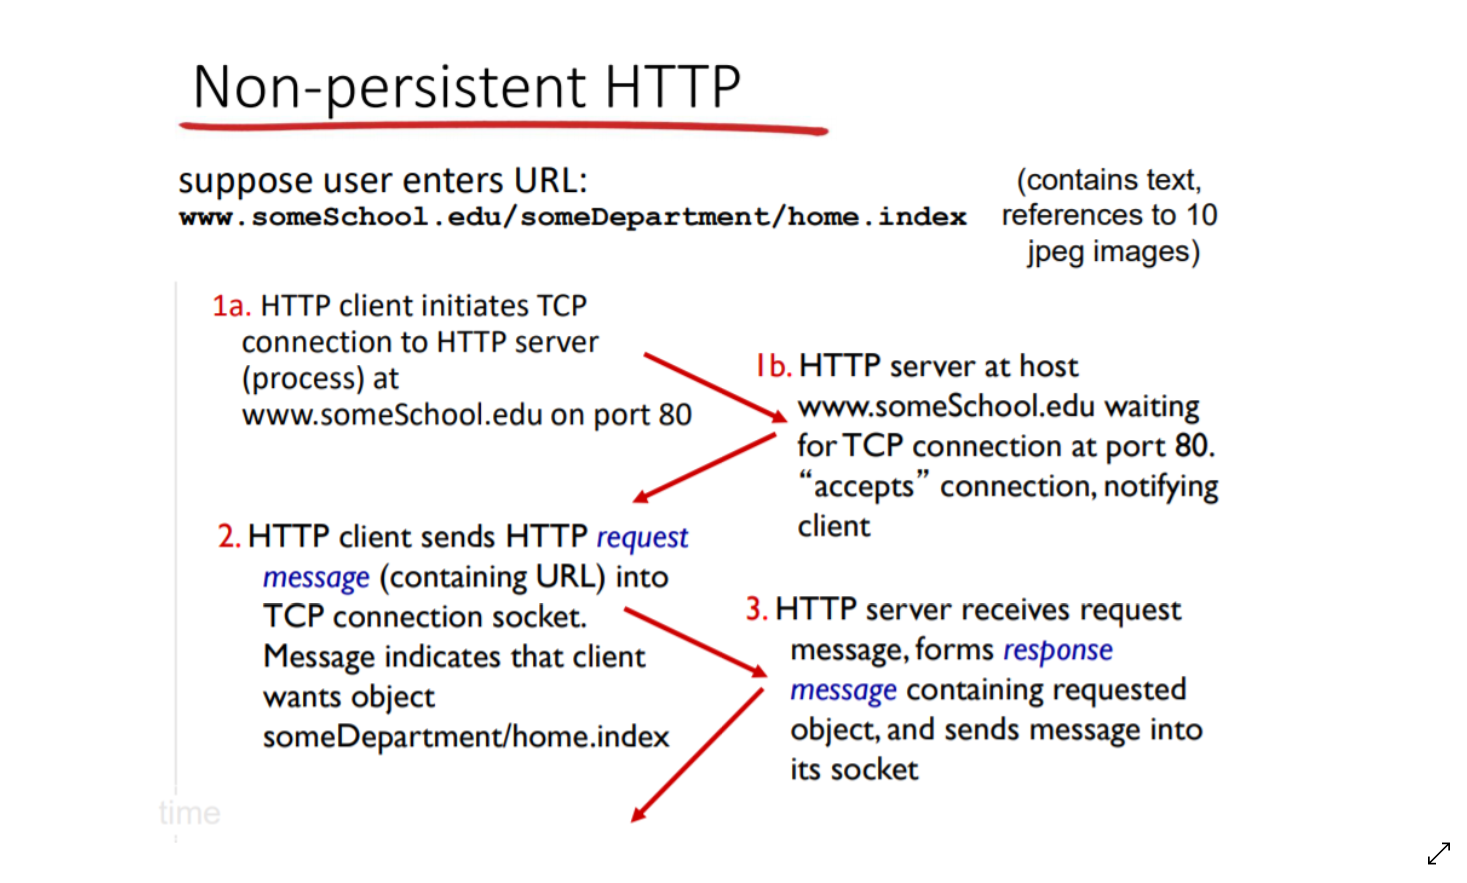
\includegraphics[width=\textwidth]{image/myfolder/np.png}
    \caption{process step one}
     \*
    \centering
    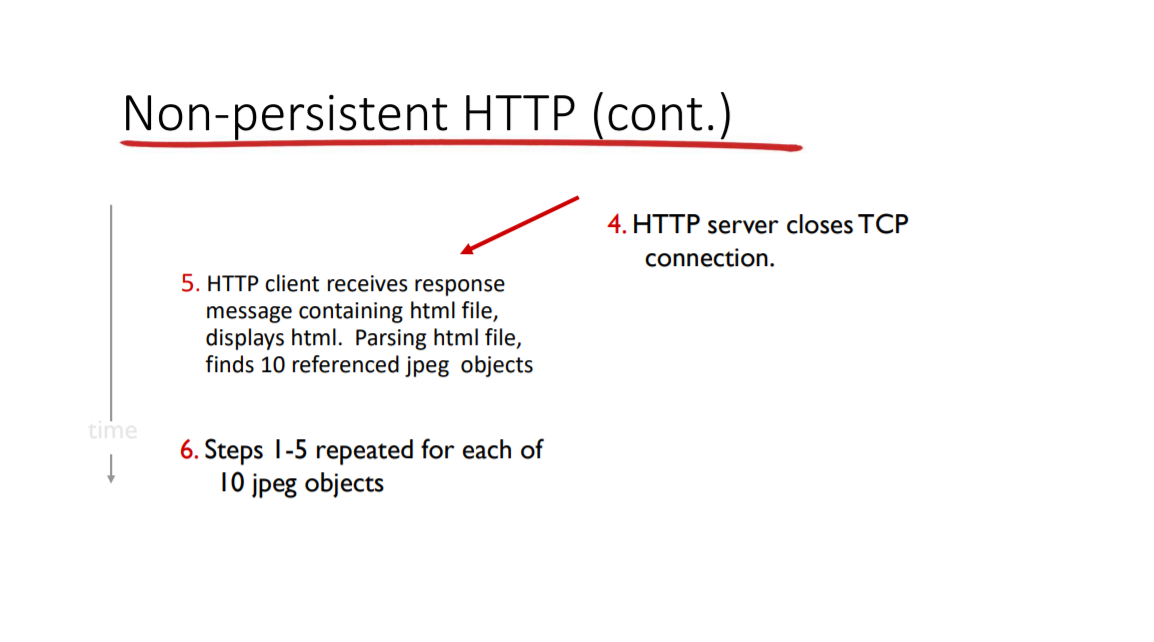
\includegraphics[width=\textwidth]{image/myfolder/np2.png}
    \caption{process step two}
\textbf{None Persistence Http: Response Time}
    \centering
    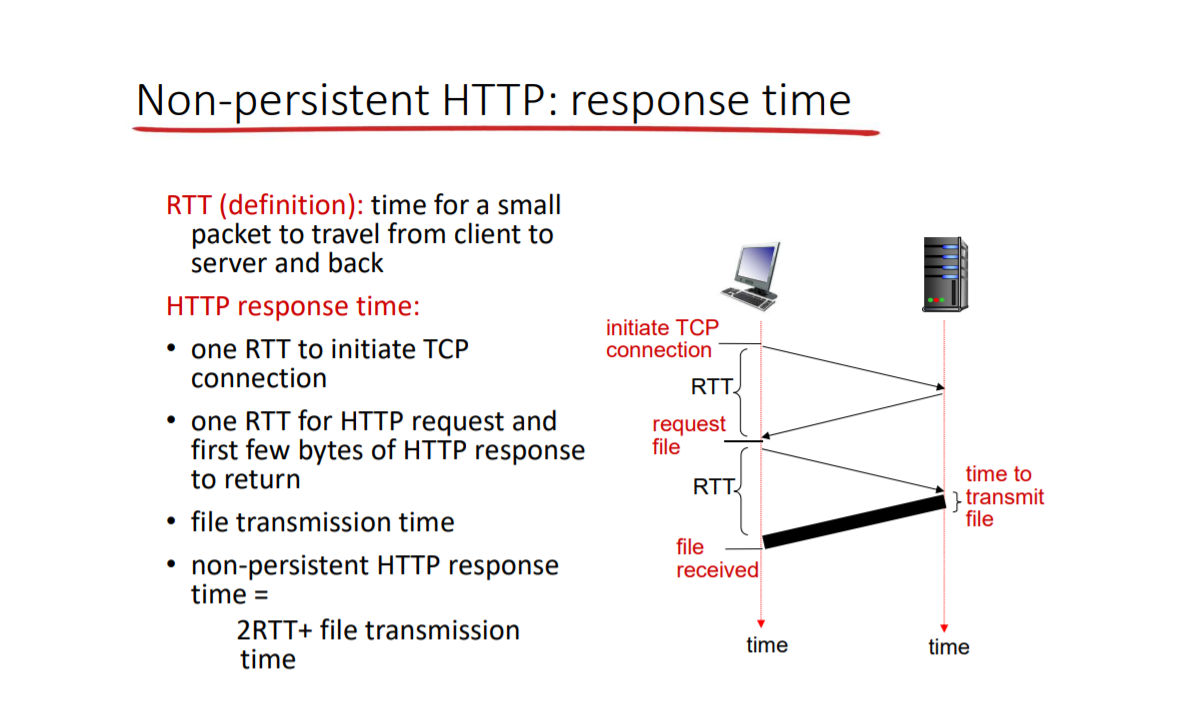
\includegraphics[width=\textwidth]{image/myfolder/np3.png}
    \caption{response time}
\end{figure}
\vfill
\clearpage



\subsection{Persistent HTTP VS Non-Persistent HTTP}
\textbf{Non-persistent HTTP issues:}
\begin{itemize}
\item requires 2 RTTs per object
\item OS overhead for each TCP
connection
\item browsers often open
parallel TCP connections to
fetch referenced objects
\end{itemize}
\*
\textbf{Persistent HTTP}
\begin{itemize}
\item server leaves connection
open after sending
response
\item subsequent HTTP
messages between same
client/server sent over
open connection
\item client sends requests as
soon as it encounters a
referenced object
\item as little as one RTT for all
the referenced objects, plus one RTT to start the connection, which you can also see in the Non-persistent http section above.
\end{itemize}

\par It seems that persistent HTTP is better than Non-persistent which is not true.
The combination of the two will be the best. Example will show in the next subsection: Web Applications

\subsection{Web Applications}
Web Browsers:
\begin{itemize}
\item Netscape Navigator, Internet Explorer,
\item Firefox, Chrome,
\item Opera, Edge, Safari
\item Lynx (a text-based browswer)
\end{itemize}

Web Servers
\begin{itemize}
\item Apache
\item Nginx
\item Microsoft Internet Information Server
\end{itemize}

\subsection{N ways to make the Web Applications faster}
\begin{itemize}
\item 1.CDN (CDN makes the request more efficient by sending the request to the closest server for the client)
\item 2.Proxy (A server that received the request and forward to the root server, if it can't serve the request itself, which means it can't find the page in its cache)
\item 3.Local server (server that host in your local private network), this is the fastest server, because the connection to the public network have a bottleneck(Speed limit for the network), but local servers have a much higher limit, but it may not have all the thing you want. But this is best we can do.
\item 4. Using persistent HTTP:
total RTT will be: N+1 , where N is the number of reference objects it needs.
\item 5.Using parallel Non-Persistent HTTP/without pipelined: Nowadays, normally a browser can open 10 TCP at in the same time. So it will be 2 RTT, if there are 10 object.
\item 6. Using pipeline,so we can send everything in One RTT ideally. However, this may not be the choice, so we compress the object and sends a portion together in one response.
\item 7. Browser cache the object. This may have different cache strategy in different browsers.
\end{itemize}
\*
\par In conclusion, we can use parallel persistent HTTP + pipelining and compressing to get the object more faster. Using Web caching to decrease the number of time we need to send the request to server. Using CDN + Proxy + Local server to handle the request much faster and efficient and robust.


\newpage
\vfill
\begin{table}[t]
\centering
\begin{tabular}{l|l|l|}
\cline{2-3}
 & \multicolumn{1}{c|}{\textbf{GET}} & \multicolumn{1}{c|}{\textbf{POST}} \\ \hline
\multicolumn{1}{|l|}{\textbf{Restrictions}} & \begin{tabular}[c]{@{}l@{}}Only ASCII characters allowed.\\ Has limited info it can send\end{tabular} & Binary data allowed \\ \hline
\multicolumn{1}{|l|}{\textbf{Security}} & Less secure since data is in URL & \begin{tabular}[c]{@{}l@{}}More secure. Not stored in browser\\ history or logs\end{tabular} \\ \hline
\multicolumn{1}{|l|}{\textbf{Usability}} & Not for sensitive information & \begin{tabular}[c]{@{}l@{}}Used when sending passwords \\ or other sensitive information.\end{tabular} \\ \hline
\multicolumn{1}{|l|}{\textbf{Visibility}} & \begin{tabular}[c]{@{}l@{}}Visible to everyone \\ (in address bar/URL)\end{tabular} & Not displayed in address bar/URL \\ \hline
\multicolumn{1}{|l|}{\textbf{Cached}} & Can be cached & Not cached \\ \hline
\end{tabular}
\end{table}

\subsection*{REST}

Traditional web - full page reload, mostly owner-generated content
New world: lots of small requests, interaction within a page, mostly user-generated content
A ``page'' dynamically fetches content pieces to incorporate into view
Extends to little things like gradual load of content 
while typing (google instant) or scrolling (facebook, google image search - ``progressive scroll'' or ``infinite scroll''.) 

At first, people tried to get JS to fetch small pieces of html from servers and put it somewhere on the page.
The problem however was that the server and client were still exchanging html only. The client did not have control of the representation of the data it received and it could only then pass the resulting html to a certain a part of the page.

\begin{definition}{AJAX}{}
Asynchronous Javascript and XML (AJAX) is a technique which allows browsers to make asynchronous requests. What this means is that server requests are non-blocking, and code will continue running until the request comes back, in which a callback will be called.
\end{definition}

XML-RPC...  SOAP... were attempts at creating a standard of requesting content from servers.
Used XML on both the server and the client. The server would have to parse the request, send the data in an XML format and have the client parse the response. 
This failed initially. So WSDL was created as an extension of soap. WSDL allowed the programmer to know what function calls were available on the server.
Now, SOAP is successfully used in large industries.

REST = Representational State Transfer
People came up with this to get away from the XML syntax. The mechanism is simple: The client sends a request to the server and the server responds back with raw data.
Implemented via HTTP protocol verbs. Examples: GET, POST, PUT, DELETE...

\begin{definition}{RESTful}{}
Services following REST approach are called RESTful services.
\end{definition}

JSON = Javascript Object Notation
The lack of structure in rest made people realize that some structure is good as a response they came up with JSON as an alternative to XML.
It's advantages include it being a very easy to learn and to write. Also since it is using Javascript, most modern browsers can natively parse JSON. 

\begin{note}
jQuery, vue.js
\end{note}

\subsection*{COMET}
\par COMET is a model where a HTTP connection is held between the client and server. The connection is unidirectional -- the server can only send data to the client. The main problem with comet is that the client has to open new connections if it wants to send the server more information. The upside is that the server only needs to maintain one connection instead of opening multiple to send data over time, which is less expensive.
\begin{note}
Comet was named after a dish soap brand just like Ajax...
\end{note}

\subsection*{WebSockets}

\begin{note}
Traditional HTTP request
Client sends a request and wait
Server does not respond until new data is available
Server sends back data
Client receives the data and send another request
\end{note}

COMET - problem: web browsers limit number of connections
Work around: domain sharding
Since limitation is based on domain name, just use multiple domain names to open more connections
+ one way

Want two way communication between client and server - WebSockets
Provides a persistent connection and both can start sending data

\section{Cookies and Web Sessions}

Data about the user is stored on server
A session id is sent to client and stored on client
Client passes session id to server
Server uses this id to get data from the database
Persist through user's interaction with the website
Example: Google Docs
What file was being edited
where the cursor was

\begin{definition}{Cookies}{}
Small files sent from the server to be stored on client side
Used to track the client's activities and remember stateful information
First visit?
Logged-in user?
Updated on every request
\end{definition}

\par Cookies can be sent to the server by setting the Set-Cookie HTTP Response header. This will alleviate the problem of having to write convoluted GET requests with tons of parameters in the URL. Instead, we can put all the relevant data in a cookie.

\par Typically when cookies are created by the server, the information is cryptographically signed. This prevents the client from tampering with the cookie, because the server will notice the change in the signature and will ignore all the information sent if the cookie is invalid.

\begin{definition}{JWT}{}
JSON Web Token (JWT) is a standard that defines a way to transmit information between parties using a JSON object. The JWT token structure is xxxxx.yyyyy.zzzzz, which is the header, payload, and signature (respectively), separated by a dot.
\end{definition}

An example of JWT:
\begin{enumerate}
    \item When a user logs in, a JWT Token will be created server-side and saved locally in the client (cookies are also an alternative to JWT).
    \item Whenever the user wants to access a resource, the user will send the JWT token back to the server to authenticate (the token usually goes in the header).
\end{enumerate}

\par One of the differences between JWT and Cookies is that the JWT mechanism is stateless -- the server never stores user state. With cookies, the user's session must persist in the server.

\par We can actually store JWT tokens in cookies -- there are many implementations available on their website for most popular languages.

\subsection*{Server Handling of Cookies}

\par The server typically stores cookies in a database (see the Database section). Session information and related data gets put in a database, which the server will reference when the client sends information back (for both information selection and updating).

\subsection*{Web Sessions}
\par Web sessions were created to prevent malicious users from manipulating cookies. A web session is created on the server that holds a history of past connections with the client. A session is fetched by a hashed session ID which is stored on the user's client as a cookie. A single user can have multiple sessions stored on the server or even share sessions between processes. Typically modern browsers will share sessions between tabs (unless the user decides to go incognito

\par If you use different browser(Edge,Chrome,Firefox) into login to blackboard, each of the browser will open a session. If you only use one of them and open multiple tab, all the tab will have the same section, every time the session gets update. It will synchronize other tab too.

\section{Browser Caches and Request Ordering}

Caching / HEAD requests 
Performance impact due to caches and request ordering (js serialization, css FOUC)
GET vs PUT implications on caches.

Developer tools - Waterfall

\section{Domain Name System (DNS)}

\begin{definition}{Domain Name System(DNS)}{}
The Domain Name System translates domain names to IPs addresses. For example, to go to Stony Brook's website, rather than typing out the IP (http://129.49.2.176), DNS allows you to simply use http:///www.stonybrook.edu.
\end{definition}

DNS is convenient for human beings, since it's easier to remember a URL composed of words than an IP address. The process of getting a IP address from a domain name is called DNS resolution (also known as DNS lookup).

\begin{definition}{DNS Resolution/DNS Lookup}{}
DNS resolution is the process of translating an IP address to a domain name, or vice-versa. Also known as DNS lookup.

\end{definition}

Names can be pointed to new IP if server changed.
DNS records primarily A (and AAAA), but also has other helpful ones like CNAME and MX.

DNS can be fast because of lots of caching.  (Explain how DNS caching works)  Problems with caching - updates are slow (minimum 10 minutes typically enforced by public DNS servers).

DNS can also be used for geographic load balancing across datacenters.

\section{Content Delivery Network (CDN)}
CDNs are used to reduce round trip time, usually used by websites with large amounts of traffic.

\begin{definition}{Round-trip time (RTT)}{}
The amount of time it takes in milliseconds for a network request to get from its starting point to its end point. For example, the amount of time it takes for a response to be received by a client from the server after sending a request.
\end{definition}
The closer a server is to a client the shorter the RTT will be, and vice-versa. A CDN will typically consist of a network of servers in various geographical locations, where a website's data would be copied to each of these servers. The website's main server would then utilize DNS to redirect each client to the CDN server that would provided the shortest RTT, which is usually the closest server geographically. 

\chapter{Virtualization}

\begin{introduction}[Topics]
\item Virtualization
\end{introduction}

The key technology behind the cloud
Ironically, avoided by the ``biggest'' cloud systems
Software-only virtualization
VMware+qemu, long history of performance challenges
Xen ``paravirtualization'' overcame hardware limitations

Hardware-assisted virtualization
(for OS+Arch savvy: fix CPU bugs,nested page tables,SR-IOV,IOMMU)
KVM+qemu emerged (and became adopted by everyone)
Although qemu is really not a good fit...
Resurgence of paravirtualization (for performance)
On most-often used components: NIC and disk

\begin{lstlisting}
char * mem = malloc[4gb]
while true {
    run(inst)
}
run(inst) {
    switch () {
        add: (do x using registers)
        sub: (do y using registers)
        ...
        ld/st 
    }
}
\end{lstlisting}


\par One of the other problems with emulation in the beginning is that emulating the ADD/SUB commands took many commands on the software (so there was lots of overhead, making it slow) and instances competed for memory 

\par Breakthrough 1: typervisor aka virtual memory monitor (vmm) and virtual machine emulator (vme): look at chunks of assembly instructions, maybe they can be run on physical hardware - if they dont touch memory or registers then no switch statement needed! 

\par Breakthrough 2: another breakthrough: 
    instead of mapping to actual hardware, come up with virtual things! virtual disk! (with virtual driver) These work as an adaptor for the actual hardware? "Xen" came up with this. \newline
\vspace{5mm}    
    Then, Intel came up with "vmenter" "vmexit" instructions. Super fast: can't even tell you are running in vm most of the time. All vm's are run this way now.
    
\section{Virtualized Resources}


\begin{definition}{Flavor}{}
A Flavor of virtual machines has a certain amounts of the resources below (VCPU, Memory, Disk).Providers do this in order to simplify the VM selection process. OpenStack (and other provides) actually has flavors for not only different network options, but also memory, compute, storage options..
\end{definition}

\begin{itemize}
    \item latency - amount of time it takes to transfer data. generally imperceptible, and non-configurable. On the order of ms. Limited by distance (solvable with a CDN) China: 300ms. NYC: 30ms. SBU: 0ms.
    \item bandwidth - amount of data can be transferred per unit of time (order of 1-100 Gb/s) Typical cloud providers will give you 10 GB/s (or maybe 25). Servers have to have more bandwidth than the client. Not selectable in flavors: peak times = low bandwidth available, non-peak times = high bandwidth available. Torrents and porn can take up infinite bandwidth: providers will charge you for it, instead of throttling the connection
    \item aggregate transfer - GB/TB. total amount of data transferred. providers will charge you for this
    \item jitter - the variance in time delay between packets (important for interactive services like Skype -- matters less for one way videos)
\end{itemize}

\subsection*{VCPU}
VCPU - Virtual CPU dedicated to the virtual machine
This is ``virtual'' because CPU cores are time shared and not space shared; you can not physical dedicate cores from your machine to the virtual machine and never be able to access them outside your machine. In most case, 1 vCpu implies 1 thread not a actual CPU or a CPU core

\subsection*{Memory}

Memory is partitioned from the host machine

Also has the key characteristics of latency (ns), bw (GB/s), and capacity (GB). Nowadays, no one cares about latency and bw because the cpus can't keep up with the memory. We are typically limited by the computing power and bandwidth of the machine. Memory capacity is the most expensive component of a server -- it is measured in GB (typically 64 to 256). This is one of the key bottlenecks.
ECC memory
 Error-correcting code memory (ECC memory) is a type of computer data storage that can detect and correct the most common kinds of internal data corruption. ... Most non-ECC memory cannot detect errors although some non-ECC memory with parity support allows detection but not correction.


\subsection*{Disk}

Diskspace (Ephemeral vs Block)
- Ephemeral - Content is lost once machine is turned off
Block - content is persistent but more expensive as a result

Disk Space is partitioned from the host machine

There are two main types of space allocation
- Thick provision - you write 0s to all the space you are allocating to make sure you actually have that much space physically
- Thin provision - you are given an ``OK'' (there is no check); once you run out of space, virtual machine freezes until disk space frees up

\par Reasonable ranges for disks:

\begin{tabular}{ c | c | c | c }
            & Range             & SSD       & HDD \\ \hline
Latency     & 1 to 20ms         & 1ms       & 10ms \\ 
Bandwidth   & 100 to 1000MB/s   & 1GB/s     & 100MB/s \\  
IOPS        & 200k              & 200k      & 20k \\
Capacity    & 4 to 12000GB      & 1TB       & 12TB \\
Capacity/\$ &                   & 10GB/\$   & 33GB/\$\\
\end{tabular}

\subsection*{Network}

There are three main connection networks for a VM.
- Direct/Bridge - use your own network card or a physical connection
- Virtual Network - doesn't let you connect to the outside world; you can still connect to other virtual machines within your physical machine
- NAT (Network Address Translation) - Routers proxy connections from connected devices to servers (that translate source packet) and sends back responses using a lookup table

Server to Server
Typically private (different schemes on different providers, Amazon EC2, Digitalocean, Linode, ...)
Public IPs
Typically NATed (SNAT+DNAT)



\subsection{VM History}
\begin{lstlisting}
int pc;
while(true){
inst fetch(pc)
run(inst)
pc++;
}
run(init){
switch(instr opcode){
    Add: Regst[inst.dest]= Regst[inst.source1] + Regst[inst.source2]
    sub:
    Imp:
    cmp:
    ld:Regst[inst.dest] = Regst[inst.source]
    st: 
}
}
\end{lstlisting}
\par In this time the VM is very slow, because emulate one instruction is slower than running on physical hardware. So graduate student in Stanford decided that run instructions that other than LD(load),ST(store) directly using the pysical hardware. So it will be much faster, because those instruction didn't touch the memory,and not affect anything.
\*
\par however it is not fast enough for people to use. University of Cambridge led by Ian Pratt, a senior lecturer in the Computer Laboratory, and his PhD student Keir Fraser to start the project on Xen.




\par 

\subsection{Server on VM}
Many servers are run on the cloud provider's VM, and every new instance has four key features: CPU, memory, disk (OS) and net.\\*
Cloud provider doesn't let you choose those feature directly but the limited types of flavor of a VM.\\*
Ex. \\*
1  CPU   1024M   20G 1T \\*
2 CPU   2G      40G 2T\\*
4 CPU   4G      80G 4T\\*
\\*
NET:\\*
    Latency - the amount of time to transfer data\\*
    Bandwidth - the speed of data transfer per unit time\\*
    Aggregate Transfer - the actual amount of data that you transferred on your server \\*
\\*
Cloud provider usually doesn't show you their info about heir network since they have "good network" because most of the time you won't be downloading/uploading all the time (except when your server provides torrent and porn services). \\*
DISK:\\*
    \begin{itemize}
\item HDD
 
\item SSD

\end{itemize}

HDD Speed and Performance. Solid state drives (SSDs) are faster than conventional hard disk drives (HDDs) and they are also more reliable and use less power. Solid state drives have dramatically faster read and write speeds when compared with hard disk drives.


\begin{definition}{Over-provision}{}
Cloud provider proves more storage than they actually have since most of time you don't use your all of space.
\end{definition}




Memory:\\
Normally, people do talk about latency for memory because it is fast enough to keep up with the CPU.
Only people who want to over-clock or have fun, they will try to buy the "fast" memory.\\
bandwidth: GB/S\\
capacity:64GB-256GB, host:15 instance, some of the memory will be left for
other software application that runs on the server.If you run out the memory in the server(over-provision/oversubscribe),it will write to the wrong file.\\
The memory you didn't use(all of them will be use as cache), the OS will be use as a cache to give you more convenient experience. So frequently use file will be cache inside it.\\ 

CPU:A chip that fits in your computer to run program.\\

\section{Oversubscription of Resources}

Resources on a VM (cont'd)

Oversubscription/Overprovision - ``faking'' more memory than you have.
Example: allocating twenty virtual machines with 2gb RAM each when you only have 32gb of RAM on your physical machine)
- Can cause problems when physical machine runs out of memory
- Machine pages to disk when out of physical memory. This can cause massive slowdowns since performance on disk is very slow

\section{VM Features}

Lots of cool features\\
``Throw-away'' VMs\\
Suspend/Resume\\
Checkpoint/Restore\\
Clone\\
Migrate (stopped or live)\\
Cloud ``stacks''\\
EC2 - Amazon's proprietary cloud-for-rent (uses Xen)\\
Google - Google's proprietary (probably uses kvm++)\\
OpenStack - open-source choice (used by RackSpace)\\
Lots of smaller competitors (e.g., Eucalyptus, OpenNebula)\\

Cloud-specific terminology:\\
There are the terminologies used for Virtual Machines\\
Instance - a new virtual machine\\
- Flavor - defines specs such as disk space, memory, etc of virtual machine\\
- Zone - where the machine starts up\\
- Image - initial data injected into machine\\
- Migration - take one instance(disk image file) from one server move to another server\\
- live migration  - slowly copy the data into another instance, and keep track the new data that is writing to the first instance. Then after the that data has been move into second instance. you will start to move the new data that is writing when you do the live migration, and repeat the sam process until all the data is copy to the second instance.\\
You can upgrades softwares in your image to see if there would be any problem could occur so you can make sure your server won't crash.\\

\par Reasons to migrate include cloud providers who want to upgrade their own hardware -- they do a live migration, and throw away the old instance.

VM makes it very easy to do migration of your image, cloud provider copies your disk image  into another physical host. \\
Live migration uses double resources while its process, but cloud providers usually make sure only few live migrations are happening at certain time so it won't be an problem.\\
In practice, large company like Google and Amazon prefer to live migrate its cloud servers \\
One of the key feature of the VM is that, unlike physical machine, it's easy to increase size of the disk, same thing to memory.\\
It's hard to downsize your disk, because it is complicated to do that, you need to concatenate the date together, shrink it, and downsize the favor. So cloud provider typically not allow you to do that.\\

Google and Microsoft use KVM for their cloud instances, while Amazon uses Xen.

linode:\\
-the biggest fish in the small fish.(cloud provider)\\
-allow your to resize up and down for your favor.\\
Digital Ocean:\\
- does not allow to downsize.\\
SkySilk:\\
-the second biggest fish in the small fish.\\
- throw away data when resizing.\\
-does not allow you to downsize your favor.\\

Zone/Jail/Container/Serverless server:
Instances are basically resources (disk, memory, net, etc) that runs softwares.\\
Container restrict the resources on application running inside the container.\\
Most container are associated with part of the directory tree, and you can't see anything that's outside your container's directory.\\
Container starts from parent process(init, systemd) which sets up system. Then, it launches all other softwares by forking.
Container is easy to use because it's much lighter than VM and can manipulate the container easily. Deleted, add files, and set the limit on how many resources they can use.(CPU,memory,disk,etc).Everything is isolated from each other. You can modify your container from outside of your container root. It is flexible on oversubscription.\\

Issues of container:\\
It consumes some of your CPU\\
It needs a file management -> Docker is one of the solution.\\

Drawbacks of container
\begin{itemize}
    \item less secure than VMs.
    \item Fixed OS and kernel.
\end{itemize}

Serverless server: Cloud provider names it server-less server, because it is cooler in sounding(dumbest naming):, but in fact they're actually selling you a container. The main advantage of this is that they're cheaper for consumers (pricewise).\\

\par Init is a system used to bootstrap the user space and manage user processes.





\section{Containers}

\par What containers do is restrict the resources (e.g., cpu and memory limit) given to any given container. Typically OSes restrict users from using some amount of memory. The processes and files in the container are limited to itself.

\par The main advantage of a container is that you can treat them as light-weight VMs, which means you can freely destroy and do whatever you want in them.

\begin{note}
Docker is a platform which allows users to host multiple containers in a resource-efficient manner. Kubernetes helps facilitate the deployment and management of such containers. These two services can be used both independently of each other or together.
\end{note}

\section{Software development in cloud}
Unlike software designing class (CSE 308), this class will do everything pretty much the opposite. Big(O) notation isn't important in cloud software as in a normal development. Scripting language (NodeJs, Python) makes it easy to do thing,because they have a lot of third party plugins and libraries to do most of the things you want. But in the same time it lost its efficiency.
\\
Companies like Facebook, WordPress and still using PHP as their major language to develop new projects.
\\Perl - please don't read me language
\\ Companies encourage people to finish their tasks ASAP, no matter what languages they use. The result for it is that within a project there might be many languages mixed together. To make different languages work together, you make the function call to become an HTTP request and two parts of the software can communicate. If you're writing JavaScript and needs to use Python, then you can do it by starting a web server in python and accept the HTTP request from JavaScript, and use JSON to pass parameters.In this way, it also makes things easy to maintain, and replaceable. If any part break, other parts still works, if you want to rewrite part of the software you can just rewrite it in a different language. It is also faulted tolerance.\\
SOA - Server Orientated Architecture(Microservices)

\par Message broker: allows for communication between microservices through messages
\begin{itemize}
    \item Every Microservices connected to the message broker, and send the thing to it and declare the type of it. Then message broker will forward it to other Microservices.
    \item It also can queue up the message and can handle faulted tolerance, and also handle the intensive request.
\end{itemize}

This way it's easy to add and update a feature you provided\\
Microservices are running in private ip address and it's very limited so only few people can access for safety concern.

\par It's easy to get caught up in a multitude of microservices who talk to each other (in an extremely dense graph). Netflix has a good video on it, where they demonstrate how easily it is to do so.

\par A common message broker is RabbitMQ -- it primarily uses the AMQP protocol for messages, but it supports the very popular (and simple) STOMP protocol. HTTP isn't really a messaging protocol, but RabbitMQ still provides support for it.


\par Message broker normally has a "backup instance" also running in case one that is operating crash, the second one can take care of the work and the user will not feel anything. 

\section{Microservice Application Architecture}
\par Each microservice is independent of each other, so they need to have their own database, which that no one can touch it.
So when you need to change anything or rewrite the entire microservice. Everything will still work well, and you don't need to collaborate with other microservice. So each microservice will hold its own database. To avoid the overhead, you don't want a bunch of MySql/MongoDB in your instance. They will use  (CDBMS) is a database management system to take care of it.

\par Instead of having states in microservices, the general practice is to use a centralized microservice to maintain the states of the user objects, and keep other microservices stateless. 

\par In order to have a good performance server from low-performance code, there was an easy solution - buy better and more and big instances so it can handle the user's request. If you need more performance buy more and big server. 

\chapter{DevOps}

% \begin{introduction}[Topics]
% \item ...
% \end{introduction}


\section{About DevOps}

\begin{definition}{DevOps}{}
DevOps is a set of practices that automates the processes between software development and IT teams, in order that they can build, test, and release software faster and more reliably. The concept of DevOps is founded on building a culture of collaboration between teams that historically functioned in relative siloes
\end{definition}

\begin{itemize}
\item Another horribly abused term, DevOps is essentially a combination of software engineering and system administration.
\item Usually used by startups that can't afford sysadmins and DBAs, or testers
\item It's true, they can't
\item A new kind of developer environment
\item Lots of automation
\item Code deployment
\item Rollback
\item No official version numbers or release dates
\item Bug fixes and new features are gradually phased into production
\item Lots of clever tools
\item Containers for ``local'' development (Vagrant)
\item Continuous integration (and delivery)
\item Many commits and merges, constant unit testing, frequent code roll-outs
\item Jenkins
\item Configuration Management
\end{itemize}


\begin{note}
Ansible, Salt, Chef, Puppet (+git)
\end{note}

\chapter{Object Storage}

\begin{introduction}[Topics]
\item SQL Databases
\item NOSQL Databases
\end{introduction}

\section{SQL Databases}

\par SQL databases are the traditional approach to databases. They support the SQL query language, which is declarative.

\par With databases, we typically do not want to expose the database to the public. We want to make sure we never open up a database port to the public, or give it a public IP. Attackers will scan ports like 3306 (MySQL default port) to dig out your data.

\vspace{5mm}
\par \noindent Examples of popular databases:
\begin{itemize}
    \item MySQL: the most popular (free, simple, fast during conception)
    \item Postgres
    \item IBM DB2
\end{itemize}

\par \noindent Advantages of SQL:
\begin{itemize}
    \item Referential integrity
    \item Tables of structured data
    \item No duplicate key,which makes the query much faster and less things to check
\end{itemize}

\par \noindent Frameworks of SQL:
\begin{itemize}
    \item Mostly standard: DML/CRUD (INSERT, SELECT, UPDATE, DELETE)
    \item Slightly standard: Data-definition Language (DDL) (CREATE, ALTER, DROP)
    \item Non-standard: DCL - determine permissions for various objects (GRANT, REVOKE)
\end{itemize}

\par \noindent MySQL (still) wildly popular
\begin{itemize}
    \item Once was fast, but didn't always preserve data
    \item When you use it for a long time, it is hard to switch to other one for all kind of reason(don't want to pay for other database), like the example that some company still using soap(xml kind),and today we are using JSON in most of the time.
    \item "It was lacking everything that made databases good"
    \item Caught up in features (triggers, referential integrity, etc.)
    \item Lost the performance advantage even on simple cases
\end{itemize}

\newpage
\section{NoSQL Databases}

\subsection{Why use NoSQL?}

\par For cases where tables were constantly being changed (columns being added or updated), it would cause the table to freeze and prevent users from accessing it. The temporary workaround was to just have one column that contained XML or JSON, but at the point at database table started looking like HashMaps (key-value pairs). And that's exactly what NoSQL is.

\par \noindent Examples:
\begin{itemize}
    \item MongoDB
    \item CouchDB
    \item S3
    \item Riak
    \item Redis
    \item HyperDex
\end{itemize}

\par \noindent NoSQL Traits:
\begin{itemize}
    \item Schema-less (or mostly so), allows for non-uniformity and iterative development
    \item None of the cool/advanced SQL features
    \item Mostly proprietary interfaces
    \item Simple, typically less efficient (makes it ``easier'' to scale, more on this later)
    \item Several categories: key-value, document-storage, column-storage
    \item All use indexes for fast(er) retrieval
    \item Typically adapting JSON for storage and queries
    \item Many adapt HTTP/REST for communication
\end{itemize}



\chapter{Messaging}

\begin{introduction}[Topics]
\item Message Brokers
\item Brokerless Messaging
\item Efficient Messaging
\end{introduction}

Simple REST services
HTTP as back-end protocol
Synchronous
Serialization (a.k.a., ``RPC'')
JSON (pretty wasteful and inefficient, but simple)
Protobuf (the Google way)
Thrift (the Facebook way, greater language support)
Versioning of message format is important
Allows upgrading parts of the system

AMQP services
Special protocol for messaging
Asynchronous
Typically requires ``broker'' software
RabbitMQ, Kafka
Lots of options
``Durable'' queues
Consumer ``Acknowledge''
Publisher ``Confirm''
``Response'' messages via ``callback'' queues
Advanced message routing options
Typically uses publish/subscribe (pubsub) architecture
Can subscribe to specific messages or message types

\begin{note}
Thrift, Protobuf
\end{note}
\begin{note}
	Robot.txt for not crawling, only google honors it.
\end{note}



 
\chapter{Scale-Out}


\section{Scale-Out/Scale-Up}


\begin{definition}{Scale-Up}{}
Add more hardware, vertical
\end{definition}
Pros:



\begin{itemize}
\item Possibility to increase CPU/RAM/Storage virtually or physically.

\item Single system can serve all your data/work processing needs with additional hardware upgrade being done.
\item Minimal cost for upgrade

\end{itemize}
    Cons:

\begin{itemize}
\item When you are physically or virtually maxed out with limit, you do not have any other options.
\item A crash could cause outages to your business processing jobs

\end{itemize}

\begin{definition}{Scale-Out}{}
Add more servers, horizontal
\end{definition}
Pros:

\begin{itemize}
\item Load is distributed to multiple servers

\item Even if one server goes down, there are servers to handle the requests or load.
\item You can add up more servers or reduce depending on the usage patterns or load.
\item Perfect for highly available web application or batch processing operations.


\end{itemize}

Cons:
\begin{itemize}
\item You would need additional hardware /servers to support. This would increase increase infrastructure and maintenance costs.
\item You would need to purchase additional licenses for OS or required licensed software’s.


\end{itemize}
\section{Consistent Hashing}
\begin{definition}{Consistent Hashing}{}
Consistent Hashing is a distributed hashing scheme that operates independently of the number of servers or objects in a distributed hash table by assigning them a position on an abstract circle, or hash ring. This allows servers and objects to scale without affecting the overall system.
\end{definition}


\section{Sharding}

- Spread data across multiple servers

- Either client knows the home, or nodes forward request to home

- Increases read/write performance with more shards

- Spread load by horizontal scaling

- - static sharding - "everyone a-m then everyone n-z" creates imbalances. SOLUTION: Hashing

- hashed sharding - simple: hash(key)/numShards. If numShards increases, we have an issue: reassigning shards means needing to re-hash everything. SOLUTION: consistent sharding

- consistent sharding - circle of shards - each shard is responsible for a range of the keys. add or remove -->  adjust the key range. replication of shard X is shard X+1 (next shard in the circle). makes copying easier, number of keys = number of slots


\section{Replication}


-Multiple copies of data to increase read performance

-And reliability / fault-tolerance

-Writes always take place on the master

-Choice of master may depend on data

-Systems with multiple masters for data are possible

-data might not be the latest update

-Will eventually consistent but burden to maintain

-automatic fail-over


\section{Coordinate system}

-Master Slave relationship: Master write, slave read

-Write records in binary logs when write to master shard (Ex. MySQL) Then, slaves read from binary log(master), copy to local log, execute queries on log

-SQL uses SQL thread to update DB in many threads without interference and parallel, and uses IO thread to read log from master

-To change master of slaves, set a slave as master and add slaves under it

ORM - Object Relation Mapping, Ex. MySQL, NoSQL

MySQL uses Circular replication to enforce replication from only one other master, avoid time-order conflicts (two server update at same time), no conflict resolution, slow
MySQL Replication Delay – slow query in master cause delay in slaves
Solve Replication Delay -  divide into small queries, or delete in slave then delete in master
MongoDB manage shards using proxy:  detect new requests, send requests to all DB(broadcast), ensure operations are consistent, good to read heavy load, bad to write(have to add shards)
MongoDB problem: not load balanced, use Hashing to determine which shard to go to ( shard: f(key)\%N )




\section{Other}

What if you want to scale MySQL?
Master/slave replication
Read from slave, write to master
master writes to disk and writes to a binary log
slave reads the log and performs all the queries itself
To add more capacity you, create more slaves
Difficult to manage in large scale-out deployments
Led to NoSQL (MongoDB, etc.)

Object storage (persistent key value storage) (NoSQL)
Sharding and replication out of the box
Cassandra, CouchDB, MongoDB, Redis, Riak
CAP “theorem”
Applies to any system that performs writes
Consistency, Availability, Partition tolerance
Must choose two of three
Partition tolerance: split brain
Consistency: Strong, Eventual
Disconnected operation and merging conflicts
Intra-server transient failure
Offline client operation

Consistent hashing 
Why not simple hashing?
H(A) mod N     (where N is number of nodes)
If a machine is added or disappears, all data must move
Nodes organized as a ring
Hashes distributed on ring

Distributed Filesystems/Databases
Ceph, HDFS, Cassandra

- optimized for larger objects (non-img media such as videos)

- Sharding and replication out-of-the-box. Pretty much needs this for high performance reads and writes for large items




\chapter{The CAP Theory}
\section{What does CAP standards for?}

C: Consistency - if all replicas have same values\\
A: Availability - system is available\\
P: Partition tolerance - If connection within network is lost suddenly, client must still be able to reach any node\\

Considering all three properties, performance is slow.
Can only apply two of the three properties.

\section{types of commonly used databases}

relational database:\\
AC: MySQL\\

NoSql:\\
CP:Cassandra(more CP rather than AP,better performance than MongoDB in medium size application ), MongoDB\\
AP:CouchDB\\

Cassandra VS MongoDB:\\
Cassandra is good at storing data and okay at accessing data (ex. facebook use Cassandra to store those posts that nobody reads)

\chapter{Distribute file system}

\section{HDFS and Ceph}
\begin{definition}{HDFS}{}
Hadoop Distributed File System
\end{definition}
\begin{definition}{Ceph}{}
Ceph replicates data and makes it fault-tolerant,[7] using commodity hardware and requiring no specific hardware support. As a result of its design, the system is both self-healing and self-managing, aiming to minimize administration time and other costs.
\end{definition}

HDFS and CEPH Allow us to work on partial objects
HDFS assumes that files are run inside the same server

CEPH: a bit easier to bring up because the people develop ceph creates many ansible playbooks to deploy ceph.

Cases you want to store large objects:\\
\begin{itemize}
    \item Media files such as videos,pictures, musics\\

    \item Binary files such as docker images, snapshot, and virtual machine

\end{itemize}


when to use HDFS
\begin{itemize}
    \item User has more control, can optimize more, and therefore can make more mistakes
    \item User knows where the information is
    \item uses Hadoop scheduler. Take job, run job on the correct instance (user can know where this instance is), then notify the scheduler
    \item better build in error handling
\end{itemize}

when to use Ceph
% go itemize! :p
\begin{itemize}
    \item "Youll never know where your data is. the system will find it out automatically"
    \item You'll never have the ability to optimize. Ceph cluster is an all-knowing god
    \item used to be very difficult. first cloud section ever - none succeeded. Now, ansible playbooks!! so easy yay (see below)
    \itme used for backing storage for VM
    \item https://github.com/ceph/ceph-ansible
\end{itemize}


Data locality is a benefit and a burden
- HDFS embraces it, Ceph (mostly) abandons it
- Directory/metadata storage
- Centralized: Easy, but not easy to scale (HDFS NameNode)
- Decentralized: Hard, but effective (CRUSH)

all key-value based database are kinda complicated when they're distributed

\chapter{Logs and Timestamp}

You only care about logs when there's error on your program, and you want to be able to search from your log.
The common practice for people to fix bug in their programs are add more and more print statements,
but this is not readable and inefficient.
Writing logs is very performance-intensive; it consumes a lot of RAM.

2 things should be in log: What module produces the message, and the severity of the log.

\section{ Log severity levels}
\begin{itemize}
    \item Very Verbose - VVERB
    \item Verbose - VERB
    \item inform - INFO
    \item Warning - WARN
    \item Debug - DEBUG
    \item Error - ERROR
    \item Critical - CRIT
    \item Fatal - FATAL
    \item Emergency - EMERG
\end{itemize}

\begin{note}
Severity can be misleading -- some people use CRITICAL for application startup
\end{note}

\section{Log Rotation}
\noindent log rotation for handling old logs by compressing or deleting them. So you will not run out of storage.you can set the time to handle your log. If logs are getting too big, you can compress it.\\

\section{The importance of timestamp}

in linux, syslogd controls what is sent and to where based on '/etc/syslog.config'.
Syslogd – receive log msgs, write into corresponding file, include Timestamp indicate when event happened
Severity: WARN, DEBUG ERROR, INFO, CRIT, FATAL, VVERB, VERB
Log rotation: old logs get compressed, deleted, or renamed
Some systems categorize the log and write them into different log files based on the severity of the log,
so you can look at different logs for different levels or types of logging.\\
For example, checking log.error will show you log messages from error, crit and fatal.
That is, it will show things more severe than your viewed "log level"\\

On a scaled out architecture, reading logs becomes much more tedious and difficult.
As you read the logs on different machines, you look at the timestamp of the logs to see which logs correlate with each other.
However, the timing of each machine may be different from each other.\\

\noindent Synchronizing timestamps across multiple machines
\begin{itemize}
    \item centralized time - dedicate one machine to being a timer
    \begin{itemize}
        \item time keeper has to notify all machines what time is it, machines receive the time and set it to their local time 
        \item latency becomes an issue
    \end{itemize}
    \item a latency solution - send a ping, get response with latency, local datacenters to minimize latency, send many requests and asynchronously collect response, 
    garbage collector makes app slow
    \item Software to measure performance: Apache bench, Faban, K6
    \item If one of the machine is running a little bit faster than the other machines, it will synchronize its timestamp with the source(centralized time) machine by slowing down its time. Moving backwards in time could break a program.
    \item Every body should run a Network Time Protocol (NTP) service in their instance to synchronize the time.
    \item Most of the world government runs the NTP server, they are the absolute truth of time. You can't connect directly to them, because you can mount things to attack them.
    \item normally, people have multiple upper time instance to synchronize the time.
    \item you want your NTP server to be as close as to you. (ping 0.us.pool.ntp.org)

\end{itemize}

\begin{definition}{NTP}{}
The Network-Time-Protocol (NTP): A networking protocol for synchronizing clocks between computer systems
\end{definition}

Once you have your timestamps synchronized, when you have many machines set up or a randomized load balancer, it becomes too tedious to SSH into each to read the logs.
The solution is to centralize your logs into a single location. Create a single machine or micro-service to store all logs so you only have to look at one machine for your logs. Another solution is to use search indexes. Aggregate all logs to one machine on a search index.
\begin{itemize}
    \item Splunk (Costs money)
    \item Logstash with Elasticsearch + Kibana (free)
    \begin{itemize}
        \item Elastic Search : 20min to bring up Elastic Search + 5 weeks to learn Kibana.
        \item Search is pretty much build in everything that we use today.
        \item Convenient to assign unique ID to each request
        \item Pass ID and log it everywhere
        \item Many cool visualization tools to search and analyze quickly
        \item FTP – File transfer protocol
        \item Gopher protocol – extract web documents stored on web servers, page with everything 
        \item HTTP – client traverse between servers
     \end{itemize}
\end{itemize}
\section{Writing Logs}

Logs are critical in all deployments
\begin{itemize}
    \item Troubleshooting of individual events
    \item Troubleshooting of aggregate events
    \item Insight into performance and behavior aka analytics
\end{itemize}


\noindent Possible downfalls:
\begin{itemize}
    \item Variable verbosity requires care
    \item Too little logs --> cannot trace back to event of interest
    \item Not enough data to trace security incidents
    \item Too much logs --> looking for needle in haystack
    \item Too much data to find things conveniently
    \item Negative impact on performance
    \item Logs are big and consumes a lot of disk space.
    \item Logs will permanently grow and grow
    \item Reading over scaled out architectures
\end{itemize}

\noindent Possible solutions:
\begin{itemize}
    \item Consuming too much disk space; solved with log rotation - the process of taking old logs, and compressing or deleting them. 
    \begin{itemize}
        \item have to determine how long our "rotation" is. maybe 1 month?
        \item functions something like a cache: rotate out old logs into compressed, then rotate some compressed logs into deletion
        \item rotated out log file gets compressed
        \item if logfile name is "logfile", others will be "logfile.1" etc
    \end{itemize}
    \item Scaled out logs
    \begin{itemize}
        \item Timestamp in UTC with NTP
        \item Centralize logs in one place
    \end{itemize}
\end{itemize}
Splunk – a software to search, monitor, index logs, “log management”




\section{Summary}
\begin{itemize}
    \item Exists in two flavors: centralized (syslog) and roll your own
    \item Traditionally disconnected among services and machines
    \begin{itemize}
        \item Need timestamp sync to make sense of multiple logs (NTP, UTC)\item Cloud based system have to configure UTC Time Zone(default), NTP(synchronize clock)
        \item Store in centralized place (Log aggregation)
        \begin{itemize}
            \item Logstash (centralize) + Elasticsearch and Kibana (Search index)
            \item Splunk
        \end{itemize}
    \end{itemize}
    \item A common failure mode: disk full of logs
    \begin{itemize}
        \item Need to make sure rotation enabled
    \end{itemize}
\end{itemize}


\chapter{Web Searching}

\section{About}
Instead of scaling up, google decide to scale out to save money on servers. These "servers" are just a bunch of CPUs and memory put together.\\

Even before Google, searching in the cloud index is challenging due to the amount of data that relates to a search.\\

What page should appear first and how to rank them? \\
primitive search result ranking is depended on:
\begin{itemize}
    \item whether that html page has a description tag in the html header section that matches the key word;
    \item The words in the title
\end{itemize}

some people begin to cheat, to add those popular word into their title or description so they can gain the popularity in this way.

Yahoo is the largest directory sites, host a list of urls

Google – greater capacity, scale out and sharding(many cheap machines), search index, copies all websites, most relevant search result, index pages, many physical location, good recall

Some Search Engine Examples: Inktomi(bad user experience, bad page rank, no snippets, no caching), Hotbot, Altavista(first to index full text page)

How do you identify the content is relevant to what the user search?\\

search engines started to use website's reputation to arrange their ranking in the searching result.\\
ways to determine the reputation of a website:\\
\begin{itemize}
    \item traffic of the website
    \item number of links pointing to it from other websites. Popular site will have many link point to them
    \item if reputable sites link to other sites, those sites are deemed more reputable
\end{itemize}{}    

about 10 years ago, Google start to crack down on people who sold their site's reputation by manually adding those site into their black list.

selling reputation requires some semi-illegal actions, absolutely not ethical according to ACM codes
link to the ACM codes: https://www.acm.org/code-of-ethics

People in US normally will not do this, but they will pay the people in the "East" to do that.


ways to cheat today:
\begin{itemize}

    \item take contents from wiki to increases reputation
\end{itemize}{} 


the most important consideration of why Google is on top today: their search results are the most relevant.
Smaller search engines cannot index huge amount of data because they don't have enough money

location is one of the priority factor that's going to be consider during your search in order to provide more relevant result to you. \\
How do you judge whether a search result is good or bad?\\
High precision and accuracy. In most case accuracy is prefer over precision, but if there is not enough precision accuracy is useless.\\

\vfill
\graphicspath{{image/myfolder/}}
\section{Precision and Accuracy}
\begin{figure}[htp]
    \centering
    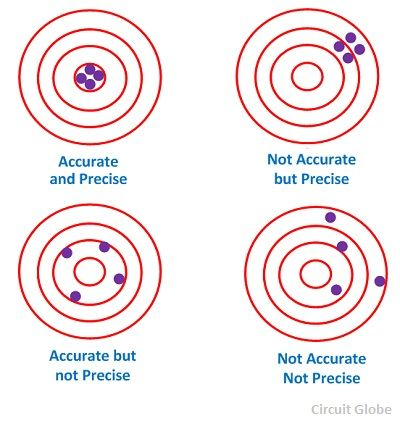
\includegraphics[width=\textwidth]{image/myfolder/searchanalogy.png}
    \caption{analogy}
     
\end{figure}
\vfill
\clearpage



what makes a search engine good:

\begin{itemize}
    \item index many things
    \item good at ranking
    \item precision of the searching result
    \item accuracy of the searching result
\end{itemize}{} 

accuracy: Accuracy is how close a measured value is to the actual (true) value.\\
precision: Precision is how close the measured values are to each other.\\
from math is fun:https://www.mathsisfun.com/accuracy-precision.html\\

precision: how much of what we got was actually relevant?\\
recall: how close we are to what we want

true positive: things appear in the correct searching result\\
false positive: wrong records that appears in the searching result\\
true negative: things shouldn't be in the searching result and it exist\\ 
false negative: things should appear in the searching result which is not\\


expectation of a searching operation:

\begin{itemize}
\item for restaurant:
        as long as it return some relevant result on the top
\item for email query:
        it's absolutely unacceptable when a email you want is not laid in the searching result
\end{itemize}


Google has generally better records than Bing, they index more site. On the other hand, Bing doesn't has that large data set and has better precision and page rank\\
If you search on Bing, chance are high the first page contains things that you care about\\
when a searching engine cross a web site, it need to create an index records all the links in the origin of that website.
creating a lookup table with token(each unique word) as its key and URL as its value\\
In a database system, create index to make query faster.\\
full-text search(inverted index): performance on the data structure called invert index,using the word(key) to find the value(URL)


Search engines today will get the full list of results and then rank.\\
Google indexes all the pages in the internet, they're storing at least one copy (usually multiple copies) for all the pages they return in their search result.\\
Google has multiple copy of nearly all of the contents of the internet, not just their index.\\
Even if the internet were to die, you can still using Google to search.\\
Google estimates how frequently a website is going to update, they use a FIFO queue to store that
relatively reputable sites will be recorded by Google once or twice a day.\\
webmaster tool : you can submit your website for indexing\\
If you don't want Google to index your site, add a robot.txt file to specify that you do not want your site indexed. Normally, third party crawler don't care this file, but Google will.
Incast Problem: Many people request to one server. Apply Node Hierarchy to load popular shards heavily, replicate more times, caching to improve performance, and queue requests
\section{Prevision vs Recall}{}
Precision and recall are two extremely important model evaluation metrics. While precision refers to the percentage of your results which are relevant, recall refers to the percentage of total relevant results correctly classified by your algorithm
\section{web crawler}{}

\begin{itemize}
    \item WebCrawler, Lycos, AltaVista, HotBot, Google 
    \item stored the whole page instead of just title, description, url
    \item Crawling to find content    \item Done frequently to notice changes
    \item Official term: Inverted Index
    \item Fast-lookup map of all elements (words) to documents
    \item May also contain location information
    \item Need to combine results for multi-word queries
    \item Precision vs Recall (email needs perfect recall, web doesn’t)
    \item Need hierarchy to query index nodes
    \item Easy features: stop words, spell check, stemming
    \item Scoring results by relevance
    \item Needs to generate result snippets (separate request)
\end{itemize}{}

DEC make the best web search engine(miss management), was bought by compaq, bought by Hewlett-Packard.\\

Google's strength: system that could have the same capacity compared to alta vista without paying millions of dollars. They bought many many cheap machines instead of one big hunk with all the information. Scaling out was the way to go. 

by extension, for the same price, they could create something with more capacity

%  \begin Page rank: Prioritize pages to show first\end

\section{Page rank} 

Why: prioritizes pages to show first 

How does page rank algo work
\begin{itemize}
    \item early on
    \begin{itemize}
        \item simplistic
        \item check for word in title, description tag
        \item later on, also check for synonyms for search term eg. hat-> cap
        \item could be gamed: invisible tag at bottom of HTML page, with random popular words at the bottom of the page
        \begin{itemize}
            \item people tried to fix this by hiring people to blacklist the websites, then with algorithms. nothing worked
        \end{itemize}
    \end{itemize}

    \item page rank algorithm uses around 120 - 150 characteristics to rank websites. One characteristic they use is the reputation of the website
    \item reputation is calculated as follows:
    \begin{itemize}
        \item number of links from other websites to our current website. The guy who started Baidu creator originally came up with this,"Google invent it 3 years afterward".
        \item take into account the reputation of the linkers to a website
        \item if 1000 disreputable websites link to you, not as meaningful as 1000 reputable websites
        \item also take into account the number of websites you are linking to. 
        \item simplistically, take your websites reputation and distribute it among everyone you link to.
        \item full algorithm is not public, has around 120 to 150 factors taken into account
    \end{itemize}
    \item Abuse of page rank – spam irrelevant keywords \item Sulution: consider reputation
\end{itemize}

\begin{definition}{Inverted index}{}
An inverted index is an index data structure storing a mapping from content, such as words or numbers, to its locations in a document or a set of documents. In simple words, it is a hashmap like data structure that directs you from a word to a document or a web page.
\end{definition}


inverted index data structure :search value to get key (opposite of regular index approach)

insertion of document in inverted index data structure via hashmap:
\begin{itemize}
  \item hash the content
  \item put hashed key as value and content as key into the hashmap
  \item if there's any data prior to current operation in the hashmap, put the hashed key into the and of the list otherwise create a new list and insert current hashed key as its first child
    \end{itemize}


prepossessing before the searching operation:

\begin{itemize}
 \item stamping
 \item spell check
\end{itemize}

Precision is the relevant fraction.
Recall is returned fraction vs total
Importance depends on context
E-mail: need perfect recall, good precision
Web: want great precision, recall is useful
Scoring is important
Usually more results than desired
Everyone wants relevance
Don’t give me what I asked for, give me what I want


Search result precision
\begin{itemize}
\item Web search split into 2 part
\item true positive:correct, false positive:false
\item others are false negative:false, true negative:correct
\item In ideal situation, search system wants true positive
\item true positive (precise), false positive(not precise)		
\item If database of search engine isn't large enough->more false negative
\end{itemize}





Whats actually inside search engine
\begin{itemize}
\item create index for all of the words and store in some datastructure
\item create lookup table for key and urls
\item Not looking for exact value of keyword. Looking for document that value came from -> fulltext search 
\end{itemize}

\begin{definition}{A/B testing}{}
A/B testing (also known as bucket tests or split-run testing) is a randomized experiment with two variants, A and B. It includes application of statistical hypothesis testing or "two-sample hypothesis testing" as used in the field of statistics. A/B testing is a way to compare two versions of a single variable, typically by testing a subject's response to variant A against variant B, and determining which of the two variants is more effective.
\end{definition}



\begin{note}
morgan is a module for node.js to monitor the request (response time etc)
https://www.npmjs.com/package/morgan

\end{note}

\chapter{Cloud Application Performance}

\begin{introduction}[Topics]
\item Tail at Scale
\item Bottlenecks 
\item Caching
\item Queuing Writes Updated
\end{introduction}


\section{Tail at Scale}{}

Average latency of request is not important as tail of latency when we looking for the QOS.
QoS dictated by the tail
X\% of requests complete in Y time
Each processing step adds latency
Client, WAN, Load Balancer, Broker, Backend, Data store
The outliers create problems at tail
QoS set at each step
Scale-out services may compound latency
Major problem for Search, MapRedce (``stragglers'')

You can use the log to track the place where the problem happens. If there are only a few slow transactions in 10000 transactions it is ok, but if 500 out of 10000 are slow, you have a problem.\\

long tail distribution:
In statistics and business, a long tail of some distributions of numbers is the portion of the distribution having many occurrences far from the "head" or central part of the distribution. The distribution could involve popularities, random numbers of occurrences of events with various probabilities, etc.[1] The term is often used loosely, with no definition or arbitrary definition, but precise definitions are possible.


peaks in the long tail distribution of latency usually are irrelevant, but tails matter

\begin{definition}{QoS}{}
Quality of service (QoS): refers to any technology that manages data traffic to reduce packet loss, latency and jitter on the network. QoS controls and manages network resources by setting priorities for specific types of data on the network.
\end{definition}

A system will always have a bottleneck, and it's hard to find the real bottleneck. It is easy to throw hardware at it to fix the problem, but you don't know where you need to "add the hardware".

Bottlenecks: there is only one real bottleneck in the system. Until you find the real bottlenecks and fix it, the performance will not improve.\\

Suppose you fix all your bottlenecks in the software, then hardware will be the problem.\\
Four type of hardware resources: Mem, CPU, net, disk.\\
Usually we don't have to worry about network bottleneck.\\
Disk bottleneck normally is causing by the log, you need to keep track of the log. Normally we avoid read and write from the disk. If we ran out of disk volume, it is easy to track.\\
CPU is the critical one\\

CPU utilization: A measure of how busy the CPU is right now.\\
Load average: number of process waiting for the CPU.\\

We intentionally keep CPU utilization low in order to provide good service.\\


\section{Bottleneck}

\begin{definition}{Bottleneck}
The single component that holds back/slows an application
\end{definition}

Since systems always have one, and only one, bottleneck at any given time, bottlenecks are not removed, they are 'shifted' aka once one bottleneck is gone, there will be a new point in your application that causes the largest slowdown.

\noindent Two types of bottlenecks:
\begin{itemize}
\item Artificial Bottlenecks
\item Hardware Bottlenecks
\end{itemize}

\begin{definition}{Artificial Bottleneck}
An artificial bottleneck is essentially a performance problem that is a direct result of a difference between the production environment or workload and the performance test environment or workload.
\end{definition}
\begin{definition}{Hardware Bottleneck}
A hardware bottleneck is the result of performance limited by a single component of hardware
\end{definition}

\noindent Artificial (Ex.):
\begin{itemize}
    \item OS kills an application once it exceeds the stack space
    \item Java: Garbage collector is slow, and as heap grows, it happens more frequently
    \item Node.js: Limited to only 1 CPU, so scaling-up can't help
    \item Flask: Also limited to 1 CPU, but isn't async like Node so each process handles requests one at a time while others wait
    \item Apache: can dynamically add/remove workers, so if initial workers too much or too little, Apache will waste time creating/killing workers
\end{itemize}

\noindent Hardware:
\begin{itemize}
    \item Net: Generally will not be a bottleneck
    \item Mem: Typically causes catastrophic failure, so easy to notice
    \item Disk: Inherently slow. Most commmon issue is leaving vverb logging on. Solving disk space is easy, simply add hardware, but disk performance issues are harder to solve. Typically done with scale-out.
    \item CPU: Add CPUs if there is a consistent CPU utilization > 60\% or Load average > the number of VCPUs
\end{itemize}
All complex systems have one bottleneck\\
Bottlenecks can shift... but there can be only one\\

Finding bottlenecks\\
Log times (and analyze them, maybe with ES)\\
Log worst-case times (and their details)\\
Monitor CPU, memory, swapping, disk, (network)?\\
``top'' is surprisingly useful\\

Fixing bottlenecks\\
Improves performance\\
Fix algorithm (e.g., cache, queue, add index, rewrite code)\\
Artificial vs Hardware bottlenecks\\
Fix config (artificial limits [app, ulimit, sysctl], features [php accelerator, pypy])\\


\section{Caching}

\begin{definition}{Caching}{}
Caching: Storing data in another location for faster read performance
\end{definition}

Mostly web static content\\
Expiration times important\\
Task can be pushed to CDN\\

Memcache: Most popular caching microservice. 
Easy to implement\\
Stores data in memory\\
Avoid redundant/duplicate computation/lookup\\
Sit in front of MySQL, ES, etc...\\
Requires invalidation on updates\\
Set expire date(usually 5 seconds)\\
Linux commands: vmstat(summary info of memory, processes, pages), iostat(cpu stat, io stat for devices)


\section{Queuing Writes}
1.when the user types a message it will appear in his/her screen, the message in the user screen may not be sent yet, the system will fix it's ordered later when it actually being sent.\\
Most online games would predict the user's action, and fix it later if it didn't happen.\\
When performing database insertion, the system would create new id when the write is entered the queue.\\
2.latency for a web is about 700ms is OK, but the fast the better.\\
3.for a phone call, the round trip time should be less than 700ms else no one can hear each other, but when they talk to each other, it will cut off each other.\\
Keep in mind:\\
sending multi-get query statements to the database requires both query statements to be independent of each other\\
You will need to wait for the entire query to finish,if you can't perform parallelism.\\
In practice, when we measure the performance of an system, we only cares about the tail of our performance graph.\\
Most of time when people look at the tail latency distribution.\\

tail latency: the slowest response time for your application \\
Look the logs from load balancer to find out who's being slow.\\

When we need/want to improve the QoS, we will like to find the bottlenecks of our application, so user can have a better experience.\\


\chapter{Security}

\begin{definition}{XSS}{}
Cross Site Scripting (XSS): An attack were the attacker injects client-side scripts into the webpage.
\end{definition}

\begin{definition}{CSRF}{}
Cross Site Request Forgery (CSRF): An attack where the attacker tricks the browser into injecting a request into an authenticated session
\end{definition}

\begin{definition}{Botnet}{}
Botnet: A network of private computers infected with malicious software and controlled as a group without the owners' knowledge, e.g., to send spam messages.
\end{definition}

\section{Security Approach}
\begin{itemize}
    \item Password Hashing: Using a hashing algorithm such as md5 or sha256 to hash passwords and store them on the database. Use with a salt so passwords are not easily guessed by looking at the hashed passwords.
    \item Server Side Code Injection: injecting code into the server. Attack happens when the server does not sanitize inputs from the client. Example: SQL Injection.
    \item Salting: concatenate some random value then hash the password. This helps to defend against Rainbow table attack in which a precomputed lookup table is used.
    \item Dangerous Assumptions: Never make assumptions about your user inputs. E.g. If a request does not have username field, do not assume this is an admin simply because you hard code the front end website to not include username field for admin login. 
    \item Botnet: To defend against botnet, make sure your machine is not compromised by code injection. Close off possible attack vectors like vulnerable ports. Do not run source files provided by the users. Professor Fredman was himself hacked this way for pulling a .php file supplied by an attacker.
\end{itemize}

\chapter{Scheduling and Job Placement}

Have lots of machines and lots of jobs
How to put the two together?
\section{Old school Approach}

Scale up as much as possible (stay on one machine)
Run things manually across machines
\section{new Approach}
use a cluster manager
Admission control, efficient task-packing, over-commit
High-availability with automatic fault-recovery time
Honors priority levels and quotas
Schedules jobs to reduce probability of correlated failures
Notable examples
Mesos, Kubernetes (similar to Borg): containers and applications
YARN: Hadoop-like resources
-	Monitor how quickly jobs are running, copy jobs to new machine to rerun
-	Wait for all jobs to finish before reduce , guess which is bottleneck
-	Decide which machine to run job
-	Less network comm, performance enhanced
-	Schedule jobs

Makespan: time from begin to terminate of jobs

Celery: simple jobs and shell scripts

\chapter{Hadoop vs Spark}
\begin{introduction}[Topics]
\item Map-Reduce
\item Hadoop
\item Spark
\end{introduction}

\section{Map-Reduce}
Another term for "Big Data"
Process lots of data, produce a (small?) aggregated result
Dominated by MapReduce pawradigm
\begin{itemize}
    \item example: counting words in a book. you can count the words one by one OR you can take 20 people, give each a page, have these people count the words on their page, then take another page
\end{itemize}
Three phases: map, shuffle, reduce
"grep" and "wordcount" are (useless?) easy examples
Easy to scale out, very fault tolerant
Many implementations
Ex.: MongoDB, CouchDB, Hadoop


\section{Hadoop}
\begin{itemize}
    \item only way to handle large data job
    \item Named after a toy elephant(author's daughter's toy)
    \item Can run in parallel(Distributed machine to run Job)
    \item Good for large-scale, not real time
    \item Comprises four main "modules"
    \item Hadoop Common, Hadoop Yarn, HDFS, MapReduce.
    \item data scientists prefer SQL, so things were made to allow SQL syntax layer above map-reduce
\end{itemize}

Libraries, GUIs
HBase, Hive, Pig, ...
Hive, Pig – query files at higher level, write SQL, return SQL output

MapReduce is great, but it is not good at doing iteration process, because it needs to write the 
output to disk and read it back again for the next iteration.So this will be time consuming. (can't to pass data between stages)
Typically used for long-running big-data batch jobs
Typically on data that takes up lots of disk space
Leverage memory and add bells and whistles
Interactive queries, stream processing, iterative execution
Careful not to step on Hadoop's toes
"Different purposes, not competitors", no other way to handle huge data, but people tend to avoid using 
hadoop as much as possible.

\section{Apache Spark}
\begin{itemize}
    \item reading data into memory, and process anything there
    \item memory is fast, so if data can fit into memory, using spark will be fast.
    \item It is design to doing things from memory, so it is very bad if you need disk I/O.
    \item cross-pollination between hadoop and spark.
    \item more likely to use this in a small company or startup.(less data)
    \item can pass output between each stage so it is very good at interactive process than Hadoop.
\end{itemize}{}


\chapter{Machine Learning}

\section{About}
new approach of programming - machine learning

efficiency in algorithms:
if rules are simple, human always do better, machine learning is good act generalization
We can't figure out the algorithm to find the correct output, and as the input gets large and large it will not be possible to do it. So we train machine learning model by feeding it the input and output to let the model learn.

Each of the input is call "feature", and each of them we will multiply by a weight.
we will learn this simple function: f(x)= w*x+b
w is the weight vector, x is the input matrix, b is a generalization term to adjust the answer, so the model will not over-fit. 

We want machines be able to learn because we can't come up with the correct algorithm.\\

overfiting : does not learn to generalize, model learns the detail that negatively impact performance and ability to generalize

type of machine learning algorithm:

\section{Types of Machine Learning}
\begin{itemize}
\item supervised: feed input with the output
\item unsupervised: feed input without the output
\item reinfoced,
\end{itemize}

\section{CNN}
CNN:
In deep learning, a Convolutional Neural Network (CNN, or ConvNet) is a class of deep neural networks, most commonly applied to analyzing visual imagery. They are also known as shift invariant or space invariant artificial neural networks (SIANN), based on their shared-weights architecture and translation in variance characteristics. They have applications in image and video recognition, recommend systems, image classification, medical image analysis, and natural language processing.


Instead treating the entire matrix as giant input, CNN takes a piece of the matrix and performance computation on it, and it can learn from those pieces 

CNN using sliding window technique, to traverse the input matrix.

Ex. Resnet, googlenet, VGG, etc.


Natural Language Processing: 

\section{Field in computer vision using CNN}
\begin{itemize}
\item object detection is the process of identification 
\item object classification is the categorization of the object based on a previously defined classes or types.
\item object segmentation is the process of splitting up an object into a collection of smaller fixed-size objects in order to optimize storage and resources usage for large objects.
\end{itemize}

\section{Embedding}
embedding in machine learning:
A word embedding is a learned representation for text where words that have the same meaning have a similar representation. It is this approach to representing words and documents that may be considered one of the key breakthroughs of deep learning on challenging natural language processing problems.
typical size of stack in a operating system is between 64 - 128 kilobytes, if something exceeds it, the operating system kills it







\chapter{Monitoring}
\section{Monitoring Programs}

    \begin{itemize}
        \item Monitoring programs detect status and report failure of micro-services. The status of a process can be running, sleeping, stopped, or zombie. Typical monitor programs monitor network services by either pretending as an user to test the correctness, expectation of output and performance, of the network services or sending ping to specific micro-services to check whether or not a specific port is open.
            
        \item Monitoring as services
        \begin{itemize}
          \item Some companies provide services that test whether or not the developing web API is functioning properly. They login to the machine and ask for data from the server. The machine runs something and send back respond either periodically or on demand.
        \end{itemize}
        
        \begin{definition}{Agent}{}
        An agent sends the data to users. Monitoring using an agent provides data regrading load average, CPU, memory utilization and network usage.
        \end{definition}
        \begin{definition}{Zenoss}{}
        A software for service monitor
        \end{definition}
    \end{itemize}
    
\section{About top}
\begin{itemize}
    \item Top
    \begin{itemize}
        \item  The top program provides a dynamic real-time view of a running system. It can display system summary information as well as a list of tasks currently being managed by the Linux kernel. The types of system summary information shown and the types, order and size of information displayed for tasks are all user configurable and that configuration can be made persistent across restarts.
        \item First column indicates the PID. Second column in top indicates how many tasks are in the system. Third column in top indicates the usage of the CPUs. 
    \end{itemize}
        

    \item htop
    \begin{itemize}
        \item a colorful top like tool with IO monitor integral within it 
    \end{itemize}
\end{itemize} 

\begin{definition}{Load Average}{}
        Reasonable percentage of load average: 60. Anything goes above 60, the tail will shift to the right. In a system that has 32 vCPUs, above 32 overloads the machine.
\end{definition}
\begin{itemize}
    \item Three details regarding load average
    \begin{itemize}
        \item id: idle, low load, high idle
        \item us: how much cup time goes to the applications
        \item If the idle percentage drop below 40 percents, some of the tasks may be queued, so the performance drop.
    \end{itemize}
\end{itemize}

\section{CPU Usage monitoring in Top}
 \begin{itemize}
        \item System load/CPU Load – is a measurement of CPU over or under-utilization in a Linux system; the number of processes which are being executed by the CPU or in waiting state.

        \item Load average – is the average system load calculated over a given period of time of 1, 5 and 15 minutes.
    \end{itemize}
    

\section{Other}
    Simple Network Protocol (SNMP): a very simple protocol expose all kinds of statistics, such as CPU and Memory utilization, and collect data from bidirectional, both client and server.


    \begin{definition}{SNMP}{}
    Simple Network Monitoring Protocol is an application–layer protocol defined by the Internet Architecture Board (IAB) in RFC1157 for exchanging management information between network devices. It always has an UID associated with the statistics that it collected.
    \end{definition}



\chapter{Homeworks}

\begin{problemset}[Homework 0 - Web Server]
	\item Create a new m.micro Linux server
    \item Assign a public IP to it and log into it
    \item Create a static web page in the server's document root called hw0.html that contains the string ``Hello World'' and one image
\end{problemset}

\begin{problemset}[Homework 1 - Ansible/Git]
    \item Place your hw0 files into a public git repository (use a service such as github or bitbucket)
    \item Create an Ansible playbook to deploy your hw0 on Ubuntu 16.04 servers, checking out the files from git and using “hw1” as the name for hosts: in your inventory
    \item Place your playbook at http://yourserver/hw1.yml
\end{problemset}

\begin{problemset}[Homework 2 - Mongodb]
	\item Install mongodb, configure it to listen to network connections
	\item Create a database called ``hw2''
	\item Create a collection called ``factbook''
	\item Populate the collection with data from https://github.com/opendatajson/factbook.json (hint: write a script to do it)
	\item Open TCP port 27017 from network 130.245.168.0/22 in the Security Group
\end{problemset}

\begin{problemset}[Homework 3 - Kubernetes]
    \item Write a dockerfile that installs a webserver and hosts hw0 on it, then build a docker image from it and host it on dockerhub.
    \item Create a single-node kubernetes cluster using minikube (m.milli instance) and deploy hw0 into it by creating a Deployment, and a Service that exposes port 80 to the Deployment. Make sure to disable virtualization with minikube by using the --vm-driver=none flag.
    \item Write a Deployment YAML (if you haven't already in the previous step) that deploys a replica of hw0 into a Pod labeled "app: hw0".
    \item Place your Deployment YAML at http://yourserver/hw3.yml.
\end{problemset}

\begin{problemset}[Homework 4 - RabbitMQ]
    \item Install rabbitmq
    \item Create a direct exchange called "hw4"
    \item Create a REST service
\begin{lstlisting}
/listen { keys: [array] }
\end{lstlisting}
Creates an exclusive queue, binds to ``hw4'' with all provided keys, waits to receive a message and returns it as
\begin{lstlisting}
{ msg: }
\end{lstlisting}
    \item Create a REST service
\begin{lstlisting}
/speak { key:, msg: }
\end{lstlisting}
Publishes the message to exchange ``hw4'' with the provided key
\end{problemset}

\begin{problemset}[Homework 5 - Load balancer]

\item Install nginx
\item Configure it as a round-robin reverse proxy between three backends:\\
http://grading.cse356.compas.cs.stonybrook.edu:9000/ \\
http://grading.cse356.compas.cs.stonybrook.edu:9001/ \\
http://grading.cse356.compas.cs.stonybrook.edu:9002/
\item Make sure failures of a backend server (e.g., timeouts or 50X responses) are not fatal and allow the other backends to handle requests
\end{problemset}

\begin{problemset}[Homework 6 - Cassandra]
\item Install Cassandra
\item Create ``hw6'' keyspace (replication factor 1)
\item Create a table "imgs" that includes a filename (string) and contents (blob) columns
\item Create a POST form target
\begin{lstlisting}
/deposit { filename: (type=text), contents: (type=file) }
\end{lstlisting}
Uploaded files should be deposited into hw6/imgs in Cassandra
\item Create a GET service
\begin{lstlisting}
/retrieve { filename: }
\end{lstlisting}
to get the previously uploaded image (make sure to respond with the appropriate image/… content type)\\
(note: use Cassandra 2.2 (22x) for this homework)
\end{problemset}

\begin{problemset}[Homework 7 - Elasticsearch]
\item Install Elasticsearch with Kibana (elastic version >=6x)
\item Create an index called ``hw7''
\item Populate the index with IMDB data about some relatively recent movies\\
(https://grading.cse356.compas.cs.stonybrook.edu/hw7/movies.json)\\
(hint, use a script or logstash)
\item Create a visualization to chart the top rated movie for every year and the average movie earnings for each year.\\
(note: don't forget to open the appropriate default port(s) for both Elasticsearch and Kibana in the security group settings, as we will be accessing Elasticsearch and Kibana via your-website.com:port)
\end{problemset}

\begin{problemset}[Homework 8 - MySQL/Memcached]
\item Install a mysql variant (mysql, maria, percona, ...)
\item Create a database called "hw8"
\item Create a table called "assists" and import MLS 2017 data for assists by soccer players (https://github.com/jokecamp/FootballData/blob/master/MLS/2017/assists.csv)
\item Create a REST service to access the data and return the top assisting player for a given club in the given position, and the average number of assists by all players of that club in that position
\begin{lstlisting}
GET /hw8?club=HOU&pos=M
\end{lstlisting}
to get \{ club:(string), pos:(string), max\_assists:(int or float), player:(string), avg\_assists:(int or float)\}

Note: Use a higher value of the goals scored (GS field) as a tiebreaker for players who have equal assists (A field).
\item Install memcached
\item Integrate memcached caching to speed up the REST-based service
\end{problemset}

\begin{problemset}[Homework 9 - Machine Learning with PyTorch]
\item Download the training script at:\\ https://grading.cse356.compas.cs.stonybrook.edu/hw9/avg\_model.py \\
Note: The script is based off of:  https://github.com/bentrevett/pytorch-sentiment-analysis/blob/\\master/3\%20-\%20Faster\%20Sentiment\%20Analysis.ipynb
\item Read through the repo's README and the folder's README to understand how the model is trained (and what neural network it decides to go for). Create an environment with the packages described in the repo's README. \\
Note: You may have an issue when following the original repo's instruction in doing 'spacy download en' (it outputs a Segmentation Fault). Just run the command again using 'sudo'.
\item Convert the training script into a webapp (e.g. by using a python web framework) with a POST endpoint "/predict" that queries the model to retrieve the sentiment value of a sentence. 
\begin{lstlisting}
POST /predict {"sentence":(type=string)}
\end{lstlisting}
The response should be in the form:
\begin{lstlisting}
{"result":(type=number)}
\end{lstlisting}
Note: disable training when setting it up for the post request and re-enable to train the model. Be sure to use a m.standard instance for this homework. \\
The repo's README mentions python 3.7, but python 3.6 will work fine.
\item For those using their own machines:
Train the model on your own laptop and then copy the resulting file into the instance and proceed with the assignment normally. If you train on your own machine, you must make sure that you do not train with cuda enabled. (I personally haven't tested in this instance, proceed at your own risk)
\end{problemset}
\chapter{Warm-up Projects}

\begin{problemset}[Warm-Up Project 1]
    \item Create a front page at http://yourserver/ttt/ - the page must include at least one CSS file which changes the appearance of something on the page and a POST FORM that requests and submits a field called 'name'. (The FORM ACTION should point to this page's own URL)
    \item If the page receives a POST parameter called 'name', it should output ``Hello \$name, \$date'' with the name and date filled in dynamically. (Do not use client-side JavaScript for this part)
    \item Create a REST-based Tic-Tac-Toe service at http://yourserver/ttt/play that takes as input a JSON object including a 'grid' property and returns a JSON object including a 'grid' property and a 'winner' property. The 'grid' property is an array of 9 characters, each being a space (' '), 'X', or 'O'. The 'winner' property is a single character to indicate who won.
    \item Integrate the REST-based tic-tac-toe service into your front page that starts operating when the page is loaded with a 'name' specified. (Use client-side JavaScript for this part)
\end{problemset}

\begin{problemset}[Warm-Up Project 2]
\item Develop a user-creation system validated with email
\begin{lstlisting}
/adduser, { username:, password:, email: }
\end{lstlisting}
creates a disabled user

\begin{lstlisting}
/verify, { email:, key: }
\end{lstlisting}
key sent via email (backdoor key is ``abracadabra''). The email should include the text 
\begin{lstlisting}
validation key: <key_goes_here>
\end{lstlisting}
(including the < and > characters). Optionally, IN ADDITION to a JSON POST request, you may also make this API call accept a GET request with the two parameters in the query string, to allow for a direct link from the verification email.

\item Add cookie-based session support
\begin{lstlisting}
/login, { username:, password: }
/logout
\end{lstlisting}
\item Modify your Tic-Tac-Toe REST service at http://yourserver/ttt/play to take as input a JSON object including a 'move' property to indicate on which square (0-indexed, in reading order) the human is making a move in the current game. The server should respond with a JSON object that includes a 'grid' property and a 'winner' property as in WP\#1. Making a request with { move:null } should return the current grid without making a move. Once a winning or tying move has been sent to the server, the server should consider the game completed and reset the grid.
\begin{lstlisting}
/ttt/play, { move: }
\end{lstlisting}
\item Maintain the history of previously played games by each user on the server.
\begin{lstlisting}
/listgames
to get { status:"OK", games:[ {id:, start_date:}, ...] }
\end{lstlisting}

\begin{lstlisting}
/getgame, { id: }
to get { status:"OK", grid:["X","O",...], winner:'X" }
\end{lstlisting}

\begin{lstlisting}
/getscore
to get { status:"OK", human:0, wopr: 5, tie: 10 }
\end{lstlisting}

Clarification: all of the above API calls must be POST requests with a JSON object for the request and JSON object as a response of either { status:``OK'' } or { status:``ERROR'' } (unless otherwise specified).
\end{problemset}
\clearpage

\chapter{Course Project}

\begin{problemset}[Twitter Clone]
\item Milestone 1: Oct. 22
\item Milestone 2: Nov. 5
\item Milestone 3: Nov 19
\item Milestone 4: Dec 3\\
Implement a Twitter clone. At a minimum, you must implement the \href{https://docs.google.com/document/d/1ycOO0sVB2TJOmIdwL6ow96pQj3k4-r7ptPsT93BInQ4/edit?usp=sharing}{\underline{API}} we provide. If you have comments or clarifying questions on the API, please leave them directly on the google doc.\\
\end{problemset}
\clearpage

\appendix



\chapter{Linux Basics}

\begin{introduction}[Topics]
\item Remote access
\item Permissions and privileges
\item Common commands
\item Directory structure
\item Popular server software
\end{introduction}

\begin{itemize}
\item remote access: ssh, scp, ssh keys
\item permission and privileges: file rwx, sudo, chmod, chown, su
\item file and directory operations: touch, mkdir, cd, ls, rm, cp, mv, cat, tail/-f, less
\item package managers: apt, yum
\item admin utils: systemctl
\item common web server software: apache2, nginx
\item popular web framework that works on Linux: Javascript nodejs/express, Python flask/Django, Java Spring MVC
\item directory structure:
    \begin{enumerate}
    \item /home is your user directory in which everything specific and private to only an user is kept. Everything else not in this directory are system directory and should have write permission restricted to root only. Inside home, there may be hidden .local, .etc, and other directories that perform the same functions as their system wide counterparts but specific to this user only.
	\item /etc is for storing system wide configuration files. This include application specific configuration across all users. 
	\item /var/log is for keeping all the logs. Both system applications dump their logs here. E.g. nginx and apache. 
	\item /tmp is a directory for storing temporary files and caches. These are usually gone after a reboot.
	\item /bin is for storing binaries that are needed by the operating system, most of which are preinstall, and necessary for it to be any useful. E.g. ls and mkdir should be found here. 
	\item /sbin is like the /bin except /sbin binaries usually need root permission to do its jobs properly. E.g. iptables and iwconfig. 
	\item /root is the home directory of the root user. Do not confuse this with the root directory aka / which contains every other directories and files in the Unix operating system.
	\item /usr contains many things which are system wide. These includes /usr/bin and /usr/sbin which are applications install by users and do the same things as /sbin and /bin except they are not needed by the operating system. Most of the applications install by the user from package managers should go inside here. There is also /usr/local which contains system wide user settings like desktop launchers in /usr/local/application (if you are running a Gui like gnome) and have yet more directories name /sbin and /bin. By convention /usr/local/bin and /usr/local/sbin are for storing binaries that are installed outside the package manager.
	\item /opt is exactly the same as /usr/local/bin and /usr/local/sbin, it is meant for storing binaries not installed with package manager. I personally do not use these directories and prefer to dump everything in /bin in my home directory if installing outside the package manager.  
	\item /boot contains the kernel. Best to stay away from it. Advanced user will usually mount this directory on a separate partition in case a kernel update goes horribly wrong. 
	\item /lib, /lib32, /lib64 contains all the dynamic and static linked libraries. If you code C or C++, that's where the compiler link their libraries from. 
	\item /usr/inlcude contains all the header files for various libraries. I usually manually dump all the headers of the libraries installed outside the package manager here, 
    \end{enumerate}
\item bash basics: 
    \begin{enumerate}
	\item | is piping
	\item > is direct std to output
	\item < is redirect stdin from input
	\item >> is append stdout to ouput
	\item << is append stdin from input
	\item \&\& is chaining together commands
	\item \& at the end of the command means to run command in the background
	\item fg is bring a background command to foreground
	\item jobs is to view all background commands 
    \end{enumerate}
\end{itemize}







\chapter{User-Server Interaction: Cookie}
As we know that an HTTP server is stateless. This simplifies server design
and has permitted engineers to develop high-performance Web servers that can handle thousands of simultaneous TCP connections. However, it is often desirable for a Web site to identify users, either because the server wishes to restrict user access or because it wants to serve content as a function of the user identity. For these purpose, HTTP uses cookies. Cookies, defined in [RFC 6265],
allow sites to keep track of users. Most major commercial Web sites use cookies today.

\graphicspath{{image/myfolder/}}
\section{Cookie}
\begin{figure}[htp]
    \centering
    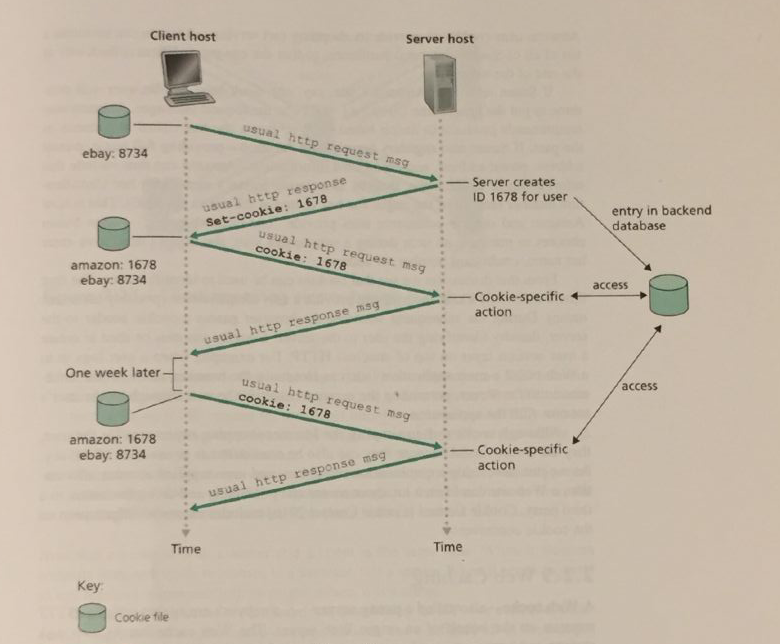
\includegraphics[width=\textwidth]{image/myfolder/cookie.png}
    \caption{cookie work flow}
\end{figure}

As show in the figure above, cookie technology has four components:
\begin{itemize}
\item 1. a cookie header line in the HTTP response message
\item 2. a cookie header line in the HTTP request message
\item 3. a cookie file kept on the user's end system and managed by the user's browser
\item 4. a back-end database at the Web site.
\end{itemize}
\*
So let's walk through an example to have a better understanding of how cookie works.

\setlength{\parindent}{10ex}
1. Suppose Tombird, who always accesses the Web using Internet Explorer from his home PC, contacts Amazon.com for the first time.Let us suppose that in the past he has already visted the eBay site. 

2. When the request comes into the Amazon Web server, the server creates a unique identification number and creates an entry in its back-end database that is indexed by the identification number.

3. The Amazon Web server then responds to Tombird's browser, including in the HTTP response a Set-cookie: header, which contains the identification number. For example, the header line might be:
Set-cookie:1678


4. When Tombird browser receives the HTTP response message, it sees the Set-cookie: header. The browser then appends a line to the special cookie file that it manages.
5. This line includes the hostname of the server and the identification number in the Set-cookie: header. Note that the cookie file already has an entry for eBay, since Tombird has visited that site in the past. 

6. As Tombird continues to browse the Amazon site, each time he requests a Web page, his browser consults his cookie file, extracts his identification number for this site, and puts a cookie header line that includes the identification number in the HTTP request. Specifically, each of her HTTP requests to the Amazon server includes the header line:
Cookie: 1678 

7. In this manner, the Amazon server is able to track Tombird's activity at the Amazon site. Although the Amazon Web site does not necessarily know Tombird's name, it knows exactly which pages user 1678 visited, in which order, and at what times!

Too be continues...




\chapter{Ansible}
\textbf{What is Ansible?}
\begin{itemize}
\item Ansible is an open-source automation tool, or platform, used for IT tasks such as configuration management, application deployment, intraservice orchestration and provisioning. Automation is crucial these days, with IT environments that are too complex and often need to scale too quickly for system administrators and developers to keep up if they had to do everything manually. Automation simplifies complex tasks, not just making developers' jobs more manageable but allowing them to focus attention on other tasks that add value to an organization. In other words, it frees up time and increases efficiency. And Ansible, as noted above, is rapidly rising to the top in the world of automation tools. Let's look at some of the reasons for Ansible's popularity.
\end{itemize}

\textbf{Advantages of Ansible?}
\begin{itemize}
\item Free. Ansible is an open-source tool.
\item Very simple to set up and use. No special coding skills are necessary to use Ansible's playbooks (more on playbooks later).
\item Powerful. Ansible lets you model even highly complex IT workflows. 
\item Flexible. You can orchestrate the entire application environment no matter where it's deployed. You can also customize it based on your needs.
\item Agentless. You don't need to install any other software or firewall ports on the client systems you want to automate. You also don’t have to set up a separate management structure.
\item Efficient. Because you don't need to install any extra software, there's more room for application resources on your server.
\end{itemize}

\textbf{Why you should use Ansible}
\begin{itemize}
\item reduce human errors.
\item time saving, one script and you can deploy as much servers as you wish
\item trackable, you can easily follow what the script is doing
\item same setup/environment for all your servers, no more "it works on my machine" problem
\end{itemize}

\chapter{Kubernetes}
\begin{itemize}
\item A Kubernetes cluster is a set of one or more machines running Kubernetes processes. A cluster has a master machine (i.e. a master node/instance) and potentially additional worker machines (i.e. worker nodes) that communicate with the master machine. All of these machines coordinate in order to manage a set of containers. For testing locally, running a Kubernetes cluster via a tool like minikube works well.
\item A Pod is a simply a contained environment that runs a docker image, i.e. a container.
\item A Deployment is for managing these Pods. it assures that a certain amount of them (i.e. an amount of replicas) are running in a certain way (e.g. what port they run on). In addition to this, you can make changes to a group of Pods via a Deployment.
\item A Service allows exposing a network to containers, thus allowing you to give a container access to ports on your public IP, e.g. http of your public IP.
\item Reference: \href{https://kubernetes.io/docs/concepts/overview/what-is-kubernetes/}{https://kubernetes.io/docs/concepts/overview/what-is-kubernetes/}
\end{itemize}







  \chapter{LaTeX Examples}

This template is based on the Standard \LaTeX{} book class, so the options of book class work as well (Note that the option of papersize has no effect due to \lstinline{device} option). The default encoding is UTF-8 while \TeX{} Live is recommended. The test environment is Win10 + \TeX{} Live 2019, either \lstinline{PDFLaTeX} or \lstinline{XeLaTeX} works fine.

\section{Definitions, Theorems, and Propositions}
section{Theorem Class Environments}

In this template, we defined four different theorem class environments

\begin{itemize}
\item \textit{Theorem Environment}, including title and content, numbering corresponding to chapter. Three types depending on the format:
   \begin{itemize}
      \item \textcolor{main}{\textbf{definition}} environment, the color is  \textcolor{main}{main};
      \item \textcolor{second}{\textbf{theorem, lemma, corollary}} environment, the color is \textcolor{second} {second};
      \item \textcolor{third}{\textbf{proposition}} environment, the color is \textcolor{third}{third}.
   \end{itemize}
\item \textit{Example Environments}, including \textbf{example, exercise, problem} environment, auto numbering corresponding to chapter.
\item \textit{Proof Environment}, including \textbf{proof, note} environment containing introductory symbol (\textbf{note} environment) or ending symbol (\textbf{proof} environment).
\item \textit{Conclusion Environments}, including \textbf{conclusion, assumption, property, remark, solution}\footnote{We also define an option \lstinline{result}, which can hide the \lstinline{solution} and \lstinline{proof} environments. You can switch between \lstinline{result=answer} and \lstinline{result=noanswer}} environment, all of which begin with boldfaced words, with format consistent with normal paragraphs.
\end{itemize}

\subsection{Theorem Class Environments}
Since the template uses the \lstinline{tcolorbox} package to customize the theorem class environments, it is slightly different from the normal theorem environments. The usage is as follows:
\begin{lstlisting}
\begin{theorem}{<theorem name>}{<label>}
The content of theorem.
\end{theorem}
\end{lstlisting}

The first parameter \lstinline{<theorem name>} represents the name of the theorem, and the second parameter \lstinline{label} represents the label used in cross-reference with \verb|ref{thm:label}|. Note that cross-references must be prefixed with \lstinline{thm:}. 

Other theorem class environments with the same usage includes:

\begin{table}[htbp]
   \centering
   \caption{Theorem Class Environments}
     \begin{tabular}{llll}
     \toprule
     Environment & Label text & Prefix & Cross-reference \\
     \midrule
     definition & label & def   & \lstinline|\ref{def:label}| \\
     theorem & label & thm   & \lstinline|\ref{thm:label}| \\
     lemma & label & lem   & \lstinline|\ref{lem:label}| \\
     corrlary & label & cor   & \lstinline|\ref{cor:label}| \\
     proposition & label & pro   & \lstinline|\ref{pro:label}| \\
     \bottomrule
     \end{tabular}%
   \label{tab:theorem-class}%
 \end{table}%
 
\subsection{Other Customized Environments}

The other three math environments can be called directly since there are no additional option for them, e.g. \lstinline{example}:
\begin{lstlisting}
\begin{example}
This is the content of example environment.
\end{example}
\end{lstlisting}

The effect is as follows:

\begin{example}
This is the content of example environment.
\end{example}

These are all similar environments with slight differences lies in:

\begin{itemize}
   \item Example, exercise, problem environments number within chapter;
   \item Note begins with introductory symbol and proof ends with ending symbol;
   \item Conclusion environment and so on are normal paragraph environments with boldfaced introductory words.
\end{itemize}

\begin{definition}{Left Coset}{}
Let $H$ be a subgroup of a group~$G$.  A \emph{left coset} of $H$ in $G$ is a subset of $G$ that is of the form $xH$, where $x \in G$ and $xH = \{ xh : h \in H \}$. Similarly a \emph{right coset} of $H$ in $G$ is a subset of $G$ that is of the form $Hx$, where $Hx = \{ hx : h \in H \}$ $\hbar$
\end{definition}

\begin{theorem}{Lagrange's Theorem}{}
Let $G$ be a finite group, and let $H$ be a subgroup of $G$.  Then the order of $H$ divides the order of $G$.
\end{theorem}

\begin{proposition}{Size of Left Coset}{}
Let $H$ be a finite subgroup of a group $G$.  Then each left coset of $H$ in $G$ has the same number of elements as $H$.
\end{proposition}

\section{Figures and Tables}

You can add Figure~\ref{fig:scatter} and Table~\ref{tab:reg} references into the text.

\begin{figure}[t]
	\centering
	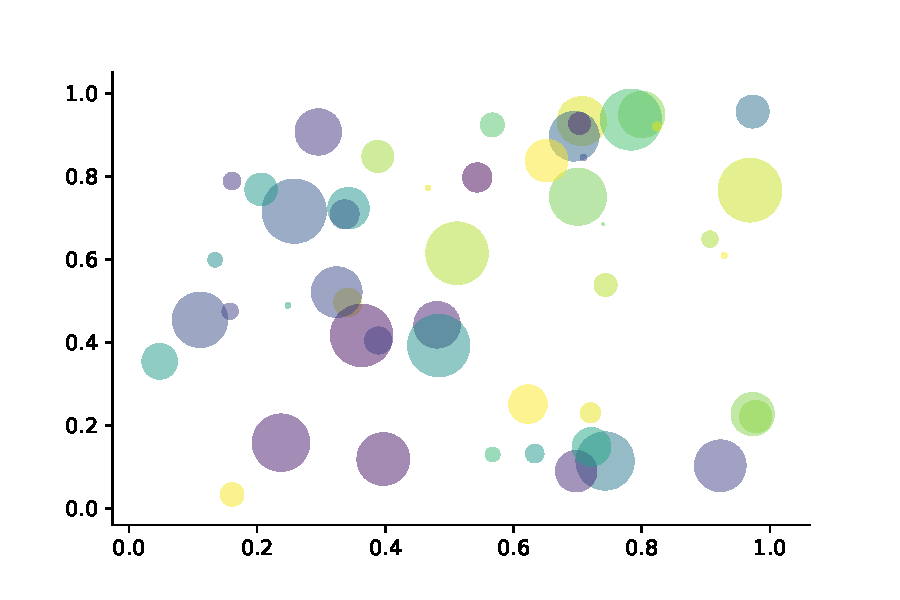
\includegraphics[width=0.6\textwidth]{figure/scatter.pdf}
	\caption{Matplotlib: Scatter Plot Example\label{fig:scatter}}
\end{figure}

\begin{table}[t]
  \small
  \centering
  \caption{Auto MPG and Price \label{tab:reg}}
    \begin{tabular}{lcc}
    \toprule
                    &       (1)         &        (2)      \\
    \midrule
    mpg             &    -238.90***     &      -49.51     \\
                    &     (53.08)       &      (86.16)    \\
    weight          &                   &      1.75***    \\
                    &                   &      (0.641)    \\
    constant        &     11,253***     &       1,946     \\
                    &     (1,171)       &      (3,597)   \\
    obs             &        74         &         74     \\
    $R^2$           &      0.220        &       0.293    \\
    \bottomrule
    \multicolumn{3}{l}{\scriptsize Standard errors in parentheses} \\
    \multicolumn{3}{l}{\scriptsize *** p<0.01, ** p<0.05, * p<0.1} \\
    \end{tabular}%
\end{table}%

\section{List Environments}

This template uses \lstinline{tikz} to customize the list environments, with \lstinline{itemize} environment customized to the third depth and \lstinline{enumerate} environment customized to fourth depth. The effect is as follows\\[2ex]
\begin{minipage}[b]{0.49\textwidth}
\begin{itemize}
   \item first item of nesti;
   \item second item of nesti;
   \begin{itemize}
      \item first item of nestii;
      \item second item of nestii;
      \begin{itemize}
         \item first item of nestiii;
         \item second item of nestiii.
      \end{itemize}   
   \end{itemize}
\end{itemize}
\end{minipage}
\begin{minipage}[b]{0.49\textwidth}
\begin{enumerate}
   \item first item of nesti;
   \item second item of nesti;
   \begin{enumerate}
      \item first item of nestii;
      \item second item of nestii;
      \begin{enumerate}
         \item first item of nestiii;
         \item second item of nestiii.
      \end{enumerate}   
   \end{enumerate}
\end{enumerate}
\end{minipage}

\subsection{Diagrams}

\begin{sequencediagram}
\newinst{ue}{UE}
\newinst[3]{nodeb}{Node B}
\newinst[3]{rnc}{RNC}
\mess{ue}{RRC Connection Request}{rnc}
\mess{rnc}{Radio Link Setup Request}{nodeb}
\mess{nodeb}{Radio Link Setup Response}{rnc}
\mess{rnc}{Establish Request}{nodeb}
\mess{nodeb}{Establish Confirm}{rnc}
\mess{rnc}{RRC Connection Setup}{ue}
\postlevel
\mess{nodeb}{Synchronization Indication}{rnc}
\filldraw[fill=black!30] ($(RRC Connection Setup to)+(0,-.3)$) rectangle ($(Synchronization Indication from) +(0,.3)$)
 node[midway] {L1 Synchronization};
\mess{ue}{RRC Connection Setup Complete}{rnc}
\end{sequencediagram}


\bibliography{reference}

\end{document}

